\documentclass[a4paper,14pt,oneside,openany]{memoir}

%%% Задаем поля, отступы и межстрочный интервал %%%

\usepackage[left=30mm, right=15mm, top=20mm, bottom=20mm]{geometry} % Пакет geometry с аргументами для определения полей
\pagestyle{plain} % Убираем стандарные для данного класса верхние колонтитулы с заголовком текущей главы, оставляем только номер страницы снизу по центру
\parindent=1.25cm % Абзацный отступ 1.25 см, приблизительно равно пяти знакам, как по ГОСТ
\usepackage{indentfirst} % Добавляем отступ к первому абзацу
%\linespread{1.3} % Межстрочный интервал (наиболее близко к вордовскому полуторному) - тут вместо этого используется команда OnehalfSpacing*

%%% Задаем языковые параметры и шрифт %%%

\usepackage[english, russian]{babel}                % Настройки для русского языка как основного в тексте
\babelfont{rm}{Times New Roman}                     % TMR в качестве базового roman-щрифта

%%% Задаем стиль заголовков и подзаголовков в тексте %%%

\setsecnumdepth{subsection} % Номера разделов считать до третьего уровня включительно, т.е. нумеруются только главы, секции, подсекции
\renewcommand*{\chapterheadstart}{} % Переопределяем команду, задающую отступ над заголовком, чтобы отступа не было
\renewcommand*{\printchaptername}{} % Переопределяем команду, печатающую слово "Глава", чтобы оно не печалось
%\renewcommand*{\printchapternum}{} % То же самое для номера главы - тут не надо, номер главы оставляем
\renewcommand*{\chapnumfont}{\normalfont\bfseries} % Меняем стиль шрифта для номера главы: нормальный размер, полужирный
\renewcommand*{\afterchapternum}{\hspace{1em}} % Меняем разделитель между номером главы и названием
\renewcommand*{\printchaptertitle}{\normalfont\bfseries\centering\MakeUppercase} % Меняем стиль написания для заголовка главы: нормальный размер, полужирный, центрированный, заглавными буквами
\setbeforesecskip{20pt} % Задаем отступ перед заголовком секции
\setaftersecskip{20pt} % Ставим такой же отступ после заголовка секции
\setsecheadstyle{\raggedright\normalfont\bfseries} % Меняем стиль написания для заголовка секции: выравнивание по правому краю без переносов, нормальный размер, полужирный
\setbeforesubsecskip{20pt} % Задаем отступ перед заголовком подсекции
\setaftersubsecskip{20pt} % Ставим такой же отступ после заголовка подсекции
\setsubsecheadstyle{\raggedright\normalfont\bfseries}  % Меняем стиль написания для заголовка подсекции: выравнивание по правому краю без переносов, нормальный размер, полужирный

%%% Задаем параметры оглавления %%%

\addto\captionsrussian{\renewcommand\contentsname{Содержание}} % Меняем слово "Оглавление" на "Содержание"
\setrmarg{2.55em plus1fil} % Запрещаем переносы слов в оглавлении
%\setlength{\cftbeforechapterskip}{0pt} % Эта команда убирает интервал между заголовками глав - тут не надо, так красивее смотрится
\renewcommand{\aftertoctitle}{\afterchaptertitle \vspace{-\cftbeforechapterskip}} % Делаем отступ между словом "Содержание" и первой строкой таким же, как у заголовков глав
%\renewcommand*{\chapternumberline}[1]{} % Делаем так, чтобы номер главы не печатался - тут не надо
\renewcommand*{\cftchapternumwidth}{1.5em} % Ставим подходящий по размеру разделитель между номером главы и самим заголовком
\renewcommand*{\cftchapterfont}{\normalfont\MakeUppercase} % Названия глав обычным шрифтом заглавными буквами
\renewcommand*{\cftchapterpagefont}{\normalfont} % Номера страниц обычным шрифтом
\renewcommand*{\cftchapterdotsep}{\cftdotsep} % Делаем точки до номера страницы после названий глав
\renewcommand*{\cftdotsep}{1} % Задаем расстояние между точками
\renewcommand*{\cftchapterleader}{\cftdotfill{\cftchapterdotsep}} % Делаем точки стандартной формы (по умолчанию они "жирные")
\maxtocdepth{subsection} % В оглавление попадают только разделы первыхтрех уровней: главы, секции и подсекции

%%% Выравнивание и переносы %%%

%% http://tex.stackexchange.com/questions/241343/what-is-the-meaning-of-fussy-sloppy-emergencystretch-tolerance-hbadness
%% http://www.latex-community.org/forum/viewtopic.php?p=70342#p70342
\tolerance 1414
\hbadness 1414
\emergencystretch 1.5em                             % В случае проблем регулировать в первую очередь
\hfuzz 0.3pt
\vfuzz \hfuzz
%\dbottom
%\sloppy                                            % Избавляемся от переполнений
\clubpenalty=10000                                  % Запрещаем разрыв страницы после первой строки абзаца
\widowpenalty=10000                                 % Запрещаем разрыв страницы после последней строки абзаца
\brokenpenalty=4991                                 % Ограничение на разрыв страницы, если строка заканчивается переносом

%%% Объясняем компилятору, какие буквы русского алфавита можно использовать в перечислениях (подрисунках и нумерованных списках) %%%
%%% По ГОСТ нельзя использовать буквы ё, з, й, о, ч, ь, ы, ъ %%%
%%% Здесь также переопределены заглавные буквы, хотя в принципе они в документе не используются %%%

\makeatletter
    \def\russian@Alph#1{\ifcase#1\or
       А\or Б\or В\or Г\or Д\or Е\or Ж\or
       И\or К\or Л\or М\or Н\or
       П\or Р\or С\or Т\or У\or Ф\or Х\or
       Ц\or Ш\or Щ\or Э\or Ю\or Я\else\xpg@ill@value{#1}{russian@Alph}\fi}
    \def\russian@alph#1{\ifcase#1\or
       а\or б\or в\or г\or д\or е\or ж\or
       и\or к\or л\or м\or н\or
       п\or р\or с\or т\or у\or ф\or х\or
       ц\or ш\or щ\or э\or ю\or я\else\xpg@ill@value{#1}{russian@alph}\fi}
\makeatother

%%% Задаем параметры оформления рисунков и таблиц %%%

\usepackage{graphicx, caption, subcaption} % Подгружаем пакеты для работы с графикой и настройки подписей
\graphicspath{{images/}} % Определяем папку с рисунками
\captionsetup[figure]{font=small, width=\textwidth, name=Рисунок, justification=centering} % Задаем параметры подписей к рисункам: маленький шрифт (в данном случае 12pt), ширина равна ширине текста, полнотекстовая надпись "Рисунок", выравнивание по центру
\captionsetup[subfigure]{font=small} % Индексы подрисунков а), б) и так далее тоже шрифтом 12pt (по умолчанию делает еще меньше)
\captionsetup[table]{singlelinecheck=false,font=small,width=\textwidth,justification=justified} % Задаем параметры подписей к таблицам: запрещаем переносы, маленький шрифт (в данном случае 12pt), ширина равна ширине текста, выравнивание по ширине
\captiondelim{ --- } % Разделителем между номером рисунка/таблицы и текстом в подписи является длинное тире
\setkeys{Gin}{width=\textwidth} % По умолчанию размер всех добавляемых рисунков будет подгоняться под ширину текста
\renewcommand{\thesubfigure}{\asbuk{subfigure}} % Нумерация подрисунков строчными буквами кириллицы
%\setlength{\abovecaptionskip}{0pt} % Отбивка над подписью - тут не меняем
%\setlength{\belowcaptionskip}{0pt} % Отбивка под подписью - тут не меняем
\usepackage[section]{placeins} % Объекты типа float (рисунки/таблицы) не вылезают за границы секциии, в которой они объявлены

%%% Задаем параметры ссылок и гиперссылок %%% 

\usepackage{hyperref}                               % Подгружаем нужный пакет
\hypersetup{
    colorlinks=true,                                % Все ссылки и гиперссылки цветные
    linktoc=all,                                    % В оглавлении ссылки подключатся для всех отображаемых уровней
    linktocpage=true,                               % Ссылка - только номер страницы, а не весь заголовок (так выглядит аккуратнее)
    linkcolor=red,                                  % Цвет ссылок и гиперссылок - красный
    citecolor=red                                   % Цвет цитировний - красный
}

%%% Настраиваем отображение списков %%%

\usepackage{enumitem}                               % Подгружаем пакет для гибкой настройки списков
\renewcommand*{\labelitemi}{\normalfont{--}}        % В ненумерованных списках для пунктов используем короткое тире
\makeatletter
    \AddEnumerateCounter{\asbuk}{\russian@alph}     % Объясняем пакету enumitem, как использовать asbuk
\makeatother
\renewcommand{\labelenumii}{\asbuk{enumii})}        % Кириллица для второго уровня нумерации
\renewcommand{\labelenumiii}{\arabic{enumiii})}     % Арабские цифры для третьего уровня нумерации
\setlist{noitemsep, leftmargin=*}                   % Убираем интервалы между пунками одного уровня в списке
\setlist[1]{labelindent=\parindent}                 % Отступ у пунктов списка равен абзацному отступу
\setlist[2]{leftmargin=\parindent}                  % Плюс еще один такой же отступ для следующего уровня
\setlist[3]{leftmargin=\parindent}                  % И еще один для третьего уровня

%%% Счетчики для нумерации объектов %%%

\counterwithout{figure}{chapter}                    % Сквозная нумерация рисунков по документу
\counterwithout{equation}{chapter}                  % Сквозная нумерация математических выражений по документу
\counterwithout{table}{chapter}                     % Сквозная нумерация таблиц по документу

%%% Реализация библиографии пакетами biblatex и biblatex-gost с использованием движка biber %%%

\usepackage{csquotes} % Пакет для оформления сложных блоков цитирования (biblatex рекомендует его подключать)
\usepackage[%
backend=biber,                                      % Движок
bibencoding=utf8,                                   % Кодировка bib-файла
sorting=none,                                       % Настройка сортировки списка литературы
style=gost-numeric,                                 % Стиль цитирования и библиографии по ГОСТ
language=auto,                                      % Язык для каждой библиографической записи задается отдельно
autolang=other,                                     % Поддержка многоязычной библиографии
sortcites=true,                                     % Если в квадратных скобках несколько ссылок, то отображаться будут отсортированно
movenames=false,                                    % Не перемещать имена, они всегда в начале библиографической записи
maxnames=5,                                         % Максимальное отображаемое число авторов
minnames=3,                                         % До скольки сокращать число авторов, если их больше максимума
doi=false,                                          % Не отображать ссылки на DOI
isbn=false,                                         % Не показывать ISBN, ISSN, ISRN
]{biblatex}[2016/09/17]
\DeclareDelimFormat{bibinitdelim}{}                 % Убираем пробел между инициалами (Иванов И.И. вместо Иванов И. И.)
\addbibresource{biba.bib}                           % Определяем файл с библиографией

%%% Скрипт, который автоматически подбирает язык (и, следовательно, формат) для каждой библиографической записи %%%
%%% Если в названии работы есть кириллица - меняем значение поля langid на russian %%%
%%% Все оставшиеся пустые места в поле langid заменяем на english %%%

\DeclareSourcemap{
  \maps[datatype=bibtex]{
    \map{
        \step[fieldsource=title, match=\regexp{^\P{Cyrillic}*\p{Cyrillic}.*}, final]
        \step[fieldset=langid, fieldvalue={russian}]
    }
    \map{
        \step[fieldset=langid, fieldvalue={english}]
    }
  }
}

%%% Прочие пакеты для расширения функционала %%%

\usepackage{longtable,ltcaption}                    % Длинные таблицы
\usepackage{multirow,makecell}                      % Улучшенное форматирование таблиц
\usepackage{booktabs}                               % Еще один пакет для красивых таблиц
\usepackage{soulutf8}                               % Поддержка переносоустойчивых подчёркиваний и зачёркиваний
\usepackage{icomma}                                 % Запятая в десятичных дробях
\usepackage{hyphenat}                               % Для красивых переносов
\usepackage{textcomp}                               % Поддержка "сложных" печатных символов типа значков иены, копирайта и т.д.
\usepackage[version=4]{mhchem}                      % Красивые химические уравнения
\usepackage{amsmath}                                % Усовершенствование отображения математических выражений 
\usepackage{listings}
\usepackage{xcolor}
\usepackage{graphicx}
\usepackage{epstopdf} %%package to overcome problem with eps in pdf files
\usepackage{amsmath}
\usepackage{amsfonts}

\usepackage{mathtools}
\usepackage{xparse}

\newcommand\tab[1][1cm]{\hspace*{#1}}

\ExplSyntaxOn
\clist_new:N \l_feq_vector_clist
\NewDocumentCommand{\feqvector}{O{\\}mO{b}}{
  \clist_set:Nn \l_feq_vector_clist {#2} % Set the list
  \begin{#3matrix}
  \clist_use:Nn \l_feq_vector_clist {#1} % show it with separator from #1 (\\)
  \end{#3matrix}
}
\ExplSyntaxOff

% \usepackage{amsthm}
% \usepackage{tcolorbox}
% \usepackage{floatrow}
% \usepackage{tabularx}
% % \usepackage[bottom]{footmisc} 
% \usepackage{titleps}
% \usepackage{breqn}
%%% Вставляем по очереди все содержательные части документа %%%

\begin{document}

\thispagestyle{empty}

\begin{center}
    МИНИСТЕРСТВО НАУКИ И ВЫСШЕГО ОБРАЗОВАНИЯ \\ РОССИЙСКОЙ ФЕДЕРАЦИИ

    \vspace{20pt}

    Университет ИТМО

    \vspace{20pt}

    Факультет систем управления и робототехники
\end{center}

\vfill

\begin{center}
    ОТЧЁТ \\  
    по лабораторной работе  №4, вариант - 2 \\
    \textit{Линейные системы автоматического управления}

    \vspace{20pt}

    по теме: \\
    \uppercase{Точностные свойства системы, астатизмы и регуляторы}
\end{center}

\vfill

\noindent Студент: \\
\textit{Группа R3336 \hfill Поляков А.А.}


    \vspace{20pt}

    \noindent Предподаватель: \\
    \textit{к.т.н., доцент \hfill  Пашенко А.В.}

\vfill

\begin{center}
    Санкт-Петербург \\ 2024
\end{center}                                     % Титульник

\newpage % Переходим на новую страницу
\setcounter{page}{2} % Начинаем считать номера страниц со второй
\OnehalfSpacing* % Задаем полуторный интервал текста (в титульнике одинарный, поэтому команда стоит после него)

\tableofcontents*                                   % Автособираемое оглавление

\label{ch:chap1}

\section{Исследование управляемости}
 
\subsection{Условие задания}

Необходимо рассмотреть систему:
$$
  \dot{x} = Ax+Bu
$$

Рассмотреть математическую модель в форме дифференциального уравнения при коэффициентах 
$a_2 = 9, a_1 = 26, a_0 = 24, b_2 = 2, b_1 = 6$, $b _0 = 8$:

\begin{gather}
	\notag
	\dddot{y} + a_2\ddot{y} + a_1\dot{y} + a_0y = b_2\ddot{u} + b_1\dot{u} + b_0u\\
	% \label{eq:dy_init}
	\dddot{y} + 9\ddot{y} + 26\dot{y} + 24y = 2\ddot{u} + 6\dot{u} + 8u
\end{gather}

% На основании полученного дифференциального уравнения \eqref{eq:dy_init} с использованием блоков элементарных 
операций построить структурную схему одноканальной линейной динамической системы.

Выполнить моделирование при входном воздействии $u(t) = 1$ и нулевых начальных условиях 
$\ddot{y}(0)$, $\dot{y}(0)$, $y(0)$.

\subsection{Решение задания}

В нашем случае имеем следующие начальные данные:
\begin{equation}
A = \begin{pmatrix}
  1 & 1 & 1 \\
  1 & 1 & 1 \\
  1 & 1 & 1 
\end{pmatrix} \tab 
B = \rowvec{a,b,c,d,e}  \tab 
x_1 = \colvec{3}{1}{0}{0}
\end{equation}


\endinput
\chapter{Наблюдатель полного порядка}
\label{ch:chap2}
\section{Условие задачи}

Рассматреть систему:
$$
  \begin{cases}
    \dot{x} = Ax \\
    y = Cx
  \end{cases}
$$ и выполнить следующие шаги:

\begin{itemize}
    \item  Найти собственные числа матрицы $A$ и определить наблюдаемость каждого из них. 
    Сделать вывод об наблюдаемости и обнаруживаемости системы.
    \item  Построить схему моделирования системы с наблюдателем состояния $\dot{\hat{x}} = A\hat{x} + L(C\hat{x}-y  )$
    \item Для каждого из спектров:
    \begin{itemize}
        \item  Найти соответствующую матрицу коррекции наблюдателя $L$, обеспечивающую желаемый спектр.
        \item Определить собственные числа матрицы наблюдателя $(A+LC)$ и сравнить
        с желаемым спектром в подтверждение корректности синтеза наблюдателя.
        \item Выполнить компьютерное моделирование с начальными условиями системы 
        $x(0) = \begin{bmatrix} 1&1&1&1 \end{bmatrix}^T$ и наблюдателя $\hat{x}(0)=\begin{bmatrix}2 & 0& 0 &-1\end{bmatrix}^T $.
        Построить  сравнительные графики $x(t)$ и $\hat{x}(t)$, а также график ошибки наблюдателя
         $e(t) = x(t) - \hat{x}(t)$
    \end{itemize}
    \item Сопоставить полученные результаты компьютерного моделирования для рассмотренных спектров, 
    оценить возможные сравнительные преимущества и недостатки каждого из них.
\end{itemize}
    

\section{Решение задачи}

Параметры для объекта:
$$
  A = \begin{bmatrix}
    -40 & 16 & 9 & -7 \\
    -64 & 25 & 14 & -12 \\
    -26 & 11 & 7 & -3 \\
    48 & -18 & -14 & 8
  \end{bmatrix} \tab
  C = \begin{bmatrix}
    -7&-2&5&-3
  \end{bmatrix}
$$
И следующие спектры сходимости для синтеза наблюдателя:
$$
  \begin{aligned}
    \sigma_1 = \{-4,-4,-4,-4\} \\
    \sigma_2 = \{-4,-40,-400,-4000\} \\
    \sigma_3 = \{-4 \pm 5i, -4 \pm 6i\} 
  \end{aligned}
$$


\subsection{Исследование наблюдаемости системы}
Найдём собственные числа матрицы $A$:
$$
    \lambda_{1,2} = \pm 3i, \tab \lambda_{3,4} = \pm 2i,
$$
Можно заметить, что тут только комплексные моды, поэтому тип вектора состояния будет иметь колебательный характер.
Найдём матрицу наблюдаемости системы:
$$
V = \begin{bmatrix}
    C \\ CA \\ CA^2 \\ CA^3
\end{bmatrix} = \begin{bmatrix}
          -7     &     -2       &    5     &     -3 \\
        134      &   -53     &    -14       &   34 \\
          28    &     53   &     -110       &   12 \\
        -1076   &      347     &     56    &    -406

            \end{bmatrix}, \tab\rightarrow rank(V) = 4
$$

В таком случае по критерию Калмана - система полностью наблюдаема , а значит и все собственные числа наблюдаемы, и как следствие - система обнаруживаема.

Рассмотрим несколько вариантов синтеза наблюдателей, с разными спектрами:

\newpage
\begin{figure}[ht]
  \centering
  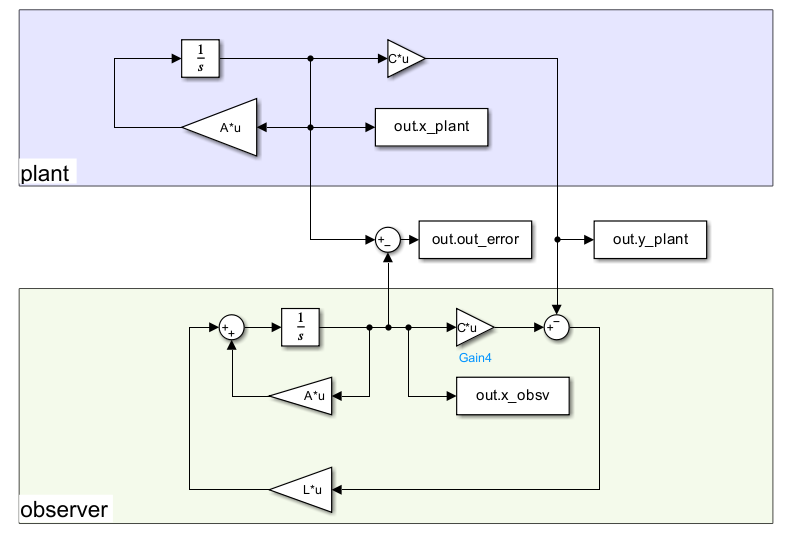
\includegraphics[width=0.8\textwidth]{model_observer.png}
  \caption{Модель с модальным наблюдателем}
\end{figure}

\subsection{Первый спектр}
$$
  \sigma_1 = \{-4,-4,-4,-4\}
$$
Система с наблюдателем полного порядка будет иметь следующие уравнения:
$$
\begin{cases}
  \dot{x} = Ax + Bu \\
  y = Cx 
\end{cases}, \tab 
\begin{cases}
  \dot{\hat{x}} = A\hat{x} + Bu +\mathbf{L}(\hat{y}-y)\\
  \hat{y} = C\hat{x} 
\end{cases}
$$

Для синтеза наблюдателя должны выполняться следующие условия:
$$
\begin{cases}
  \sigma(A)\cup\sigma(G)=\emptyset \\
  (G,Y) - \text{управляема, то всегда  существует } Q  \\
  (C,A) - \text{наблюдаема}
\end{cases}
$$
Тогда можно проследовать по алгоритму:
\begin{enumerate}
  \item Выбираем $G\in\mathbb{R}^{n\times n}$ с желаемым спектром $\sigma(G)$.
  \item Выбираем $Y\in\mathbb{R}^{n\times k}$ такую, чтобы пара $(G,Y)$ - была управляема.
  \item Найдем $Q\in\mathbb{R}^{n \times n}$ как решение уравнения Сильвестра $GQ - QA = YC$.
  \item Вычисляем матрицу коррекции наблюдателя: $L = Q^{-1}Y$
\end{enumerate}
Для получения $L$ возьмём следующую управляемую пару $G,Y$:
$$
G = \begin{bmatrix}
  -4  &   1  &   0  &   0 \\
  0  &  -4   &  1   &  0 \\
  0  &   0  &  -4  &   1 \\
  0   &  0   &  0  &  -4
\end{bmatrix}, \tab Y = \begin{bmatrix} 0\\1\\0\\1 \end{bmatrix},\tab \rightarrow \tab
L = \begin{bmatrix}
      11.08\\16.99\\9.74\\-15.62
    \end{bmatrix}
$$
Определим собственные числа матрицы наблюдателя $(A+LC)$:
$$
    \sigma_{obsv}=\{-4, -4, -4, -4 \}
$$
Однако я записал их в несколько округленном виде, поскольку мне не удалось подобрать удачный вектор $Y$, чтобы устранить такое отклонение:
$$
    \sigma_{true}=\{-4.0044, -4 + 0.0044i, -4 - 0.0044i, -3.9956 \}
$$
Но всё же погрежность здесь несколько незначительна, поэтому всё же сделаю вывод, что желаемые спектры совпали с спектром матрицы наблюдателя - синтез корректен.

Проведём моделирование, посмотрим на сравнительный график сходимости вектора состояния наблюдателя и системы, а также на их ошибку:
\newpage
\begin{figure}[ht]
  \centering
  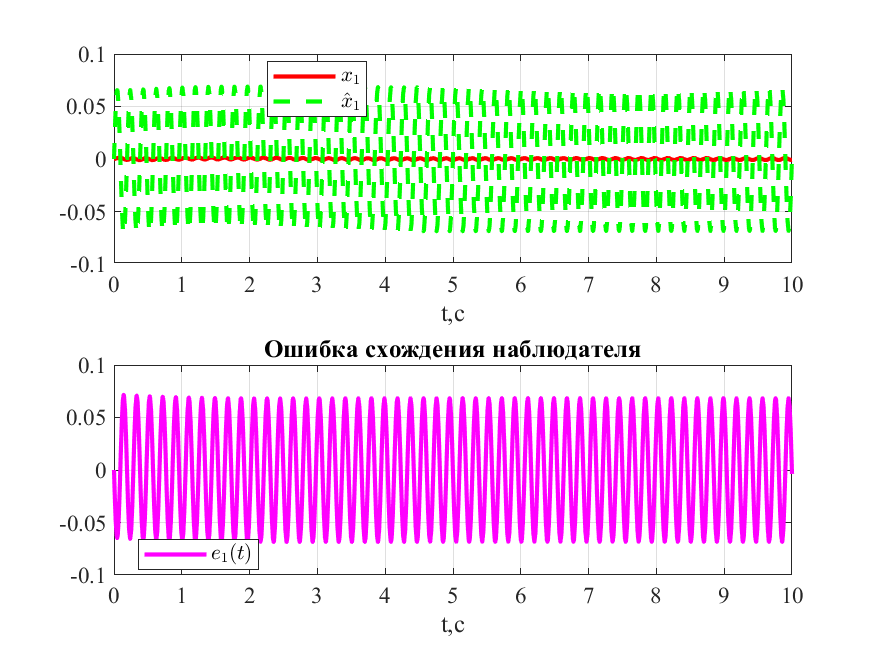
\includegraphics[width=0.8\textwidth]{obsv1.png}
  \caption{Состояние системы и ошибка сходимости}
\end{figure}
\begin{figure}[ht]
  \centering
  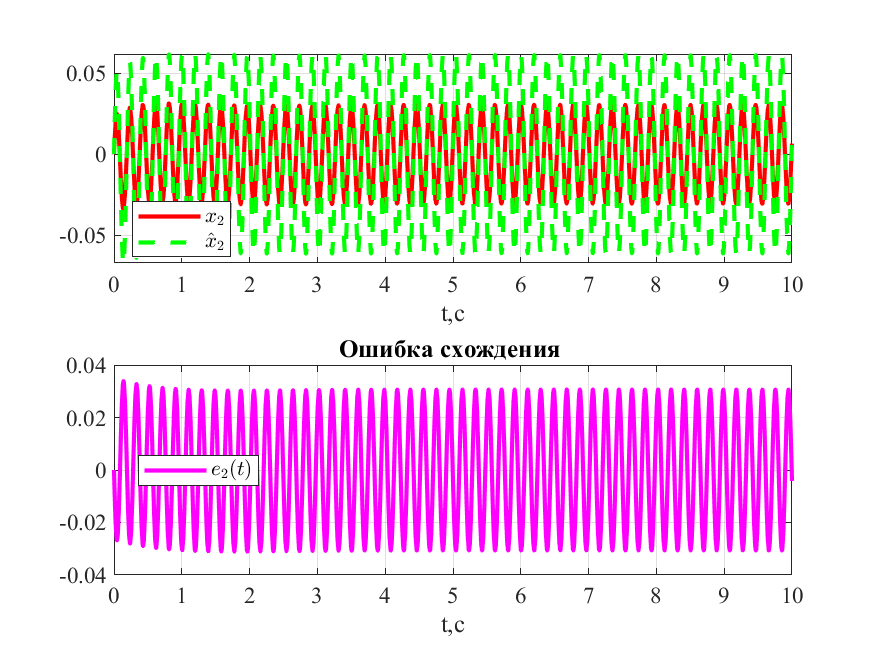
\includegraphics[width=0.8\textwidth]{obsv2.png}
  \caption{Состояние системы и ошибка сходимости}
\end{figure}
\newpage
\begin{figure}[ht]
  \centering
  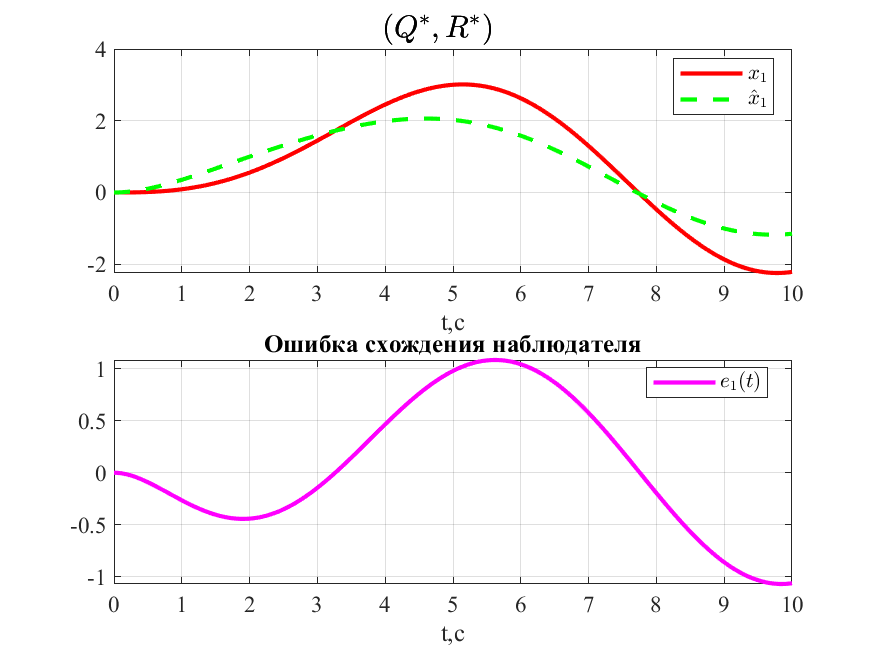
\includegraphics[width=0.8\textwidth]{obsv3.png}
  \caption{Состояние системы и ошибка сходимости}
\end{figure}
\begin{figure}[ht]
  \centering
  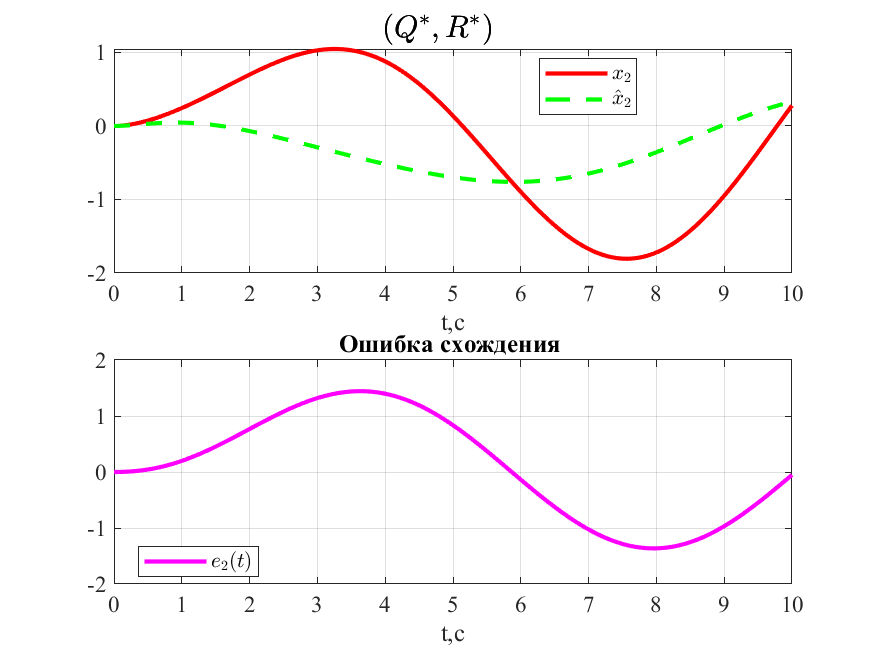
\includegraphics[width=0.8\textwidth]{obsv4.png}
  \caption{Состояние системы и ошибка сходимости}
\end{figure}


\newpage
\subsection{Второй спектр}
$$
  \sigma_2 = \{-4,-40,-400,-4000\}
$$

Для получения $L$ возьмём следующую управляемую пару $G,Y$:
$$
G = \begin{bmatrix}
  -4  &   0  &   0  &   0 \\
  0  &  -40   &  0   &  0 \\
  0  &   0  &  -400  &   0 \\
  0   &  0   &  0  &  -4000
\end{bmatrix}, \tab Y = \begin{bmatrix} 1\\1\\1\\1 \end{bmatrix},\tab \rightarrow \tab
L = 10^5\cdot\begin{bmatrix}
  3.157\\9.716\\12.754\\7.427
    \end{bmatrix}
$$
Определим собственные числа матрицы наблюдателя $(A+LC)$:
$$
    \sigma_{obsv}=\{-4, -40, -400, -4000 \}
$$
Можно сделать вывод, что желаемые спектры совпали с спектром матрицы наблюдателя - синтез корректен.
\begin{figure}[ht]
  \centering
  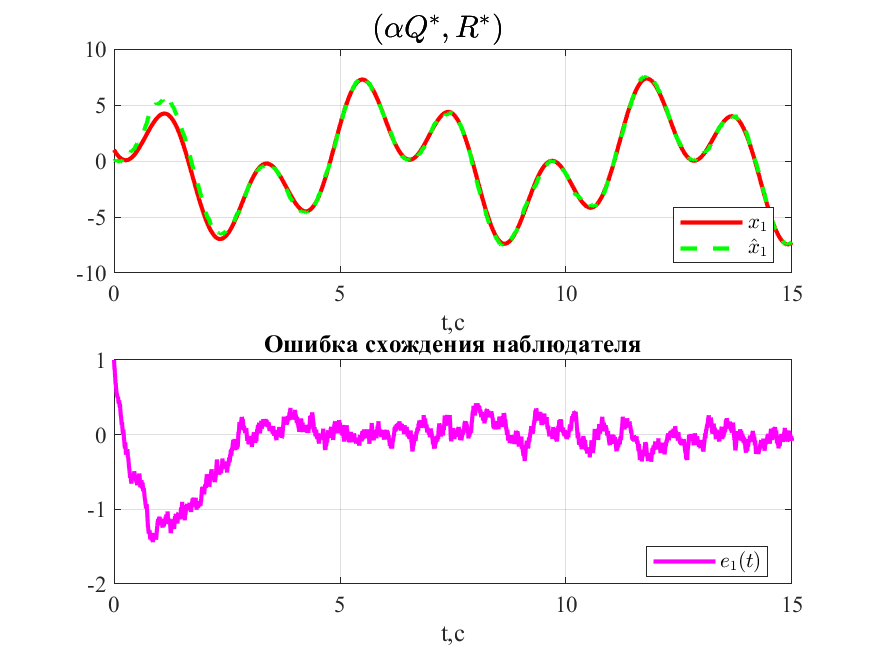
\includegraphics[width=0.8\textwidth]{obsv5.png}
  \caption{Состояние системы и ошибка сходимости}
\end{figure}
\newpage
\begin{figure}[ht]
  \centering
  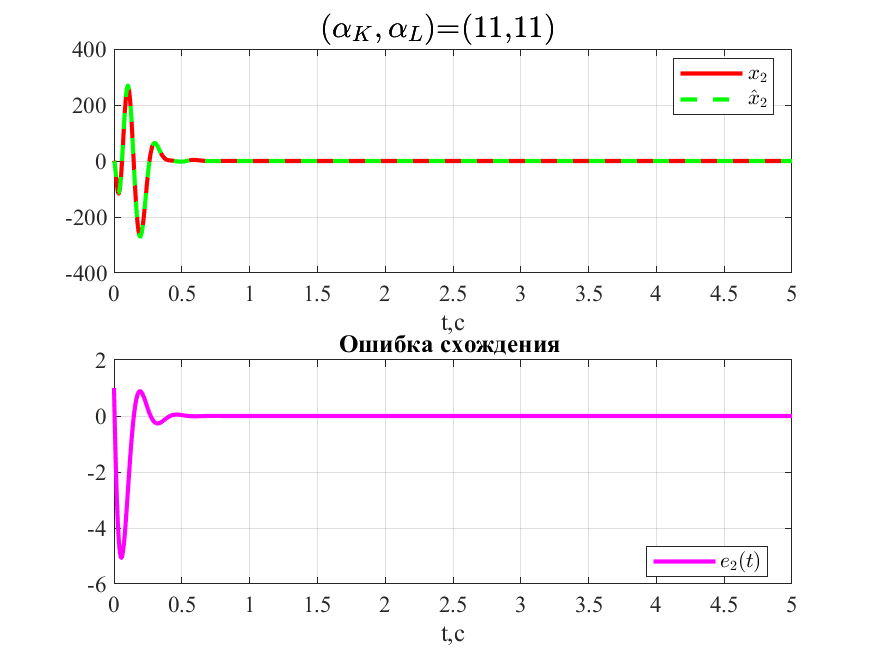
\includegraphics[width=0.8\textwidth]{obsv6.png}
  \caption{Состояние системы и ошибка сходимости}
\end{figure}
\begin{figure}[ht]
  \centering
  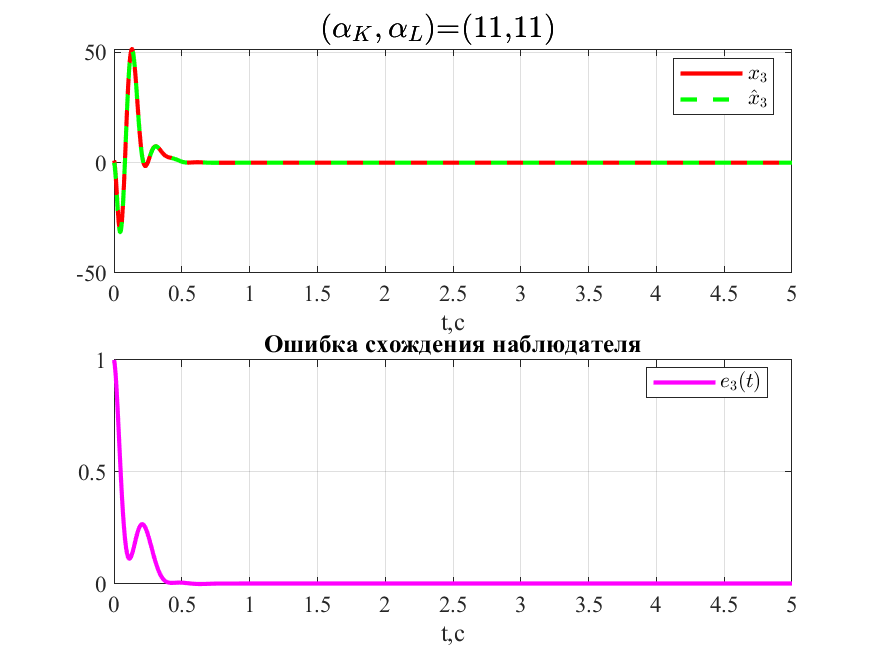
\includegraphics[width=0.8\textwidth]{obsv7.png}
  \caption{Состояние системы и ошибка сходимости}
\end{figure}
\newpage
\begin{figure}[ht]
  \centering
  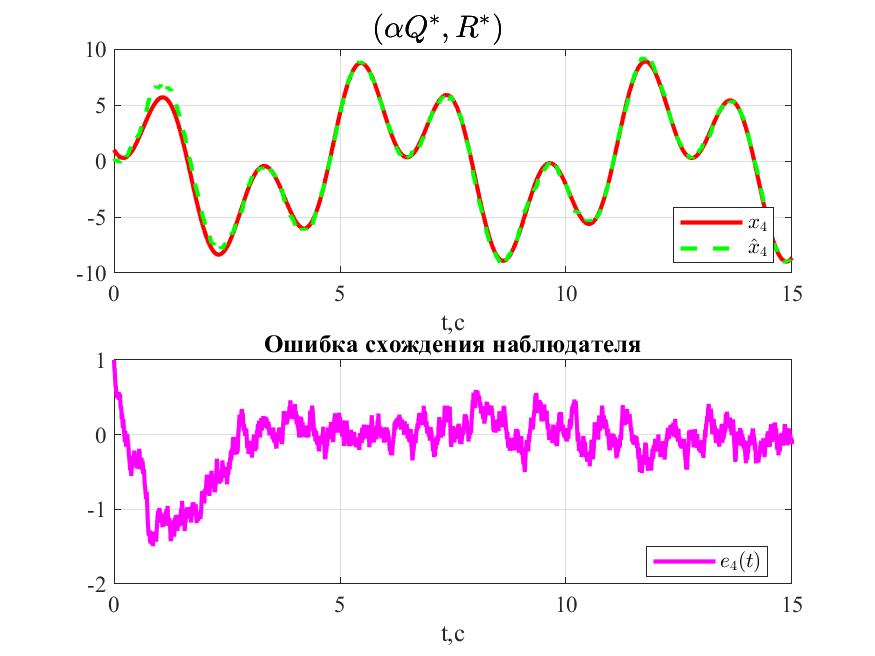
\includegraphics[width=0.8\textwidth]{obsv8.png}
  \caption{Состояние системы и ошибка сходимости}
\end{figure}


\newpage
\subsection{Третий спектр}
$$
  \sigma_3 = \{-4 \pm 5i, -4 \pm 6i\} 
$$

Для получения $L$ возьмём следующую управляемую пару $G,Y$:
$$
G = \begin{bmatrix}
  -4  &   5  &   0  &   0 \\
  -5  &  -4   &  0   &  0 \\
  0  &   0  &  -4  &   6 \\
  0   &  0   &  -6  &  -4
\end{bmatrix}, \tab Y = \begin{bmatrix} 0\\1\\0\\1 \end{bmatrix},\tab \rightarrow \tab
L = \begin{bmatrix}
  14.56\\25.87\\19.60\\-13.23
    \end{bmatrix}
$$
Определим собственные числа матрицы наблюдателя $(A+LC)$:
$$
    \sigma_{obsv}=\{-4 \pm 5i, -4 \pm 6i\}
$$
Можно сделать вывод, что желаемые спектры совпали с спектром матрицы наблюдателя - синтез корректен.
Проведём моделирование:
\begin{figure}[ht]
  \centering
  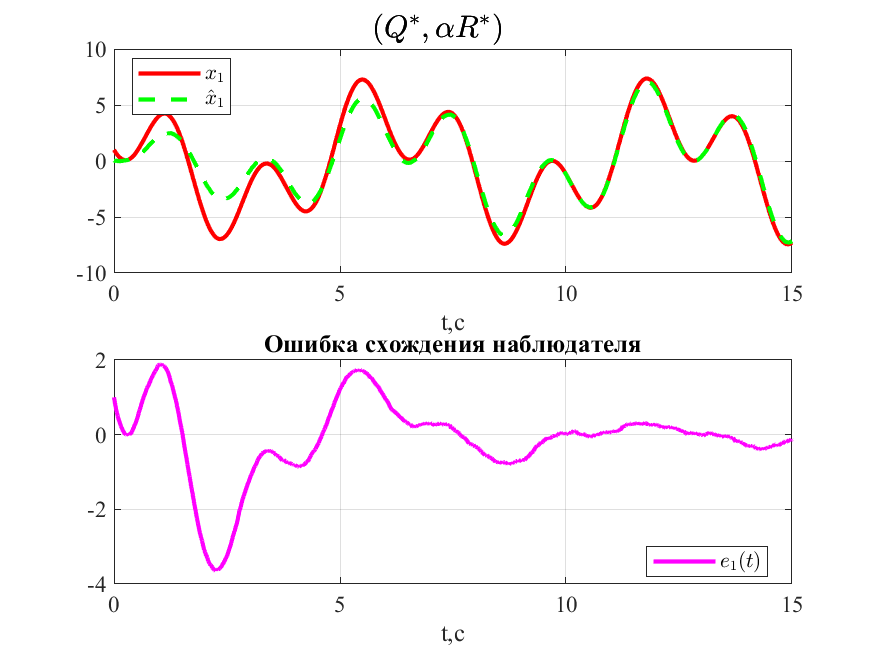
\includegraphics[width=0.8\textwidth]{obsv9.png}
  \caption{Состояние системы и ошибка сходимости}
\end{figure}
\newpage
\begin{figure}[ht]
  \centering
  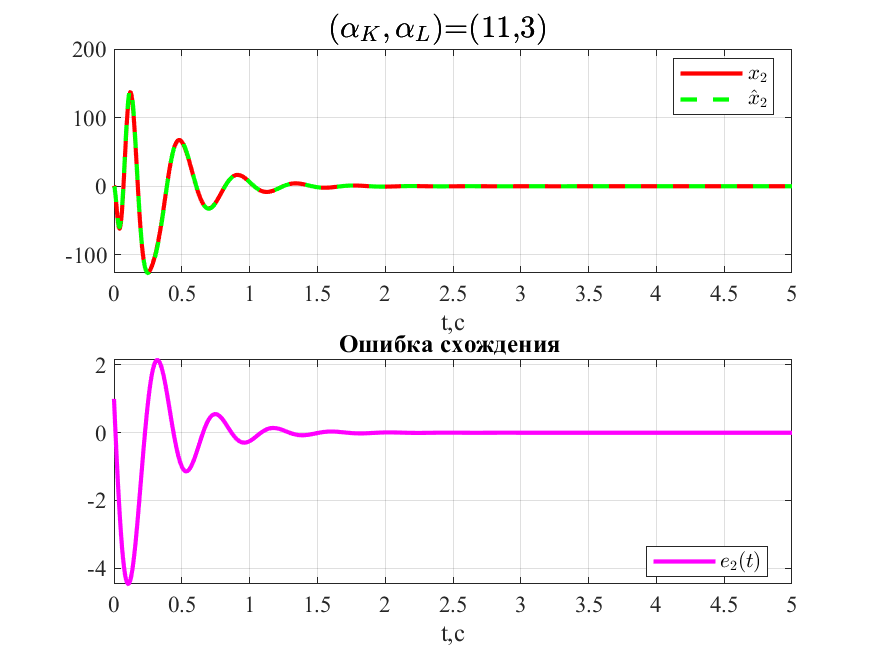
\includegraphics[width=0.8\textwidth]{obsv10.png}
  \caption{Состояние системы и ошибка сходимости}
\end{figure}
\begin{figure}[ht]
  \centering
  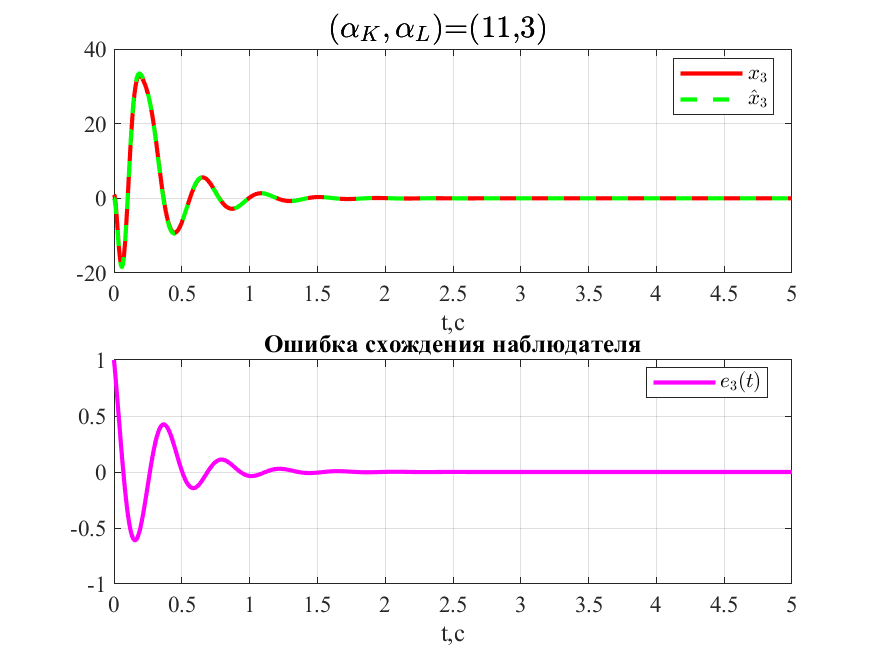
\includegraphics[width=0.8\textwidth]{obsv11.png}
  \caption{Состояние системы и ошибка сходимости}
\end{figure}
\newpage
\begin{figure}[ht]
  \centering
  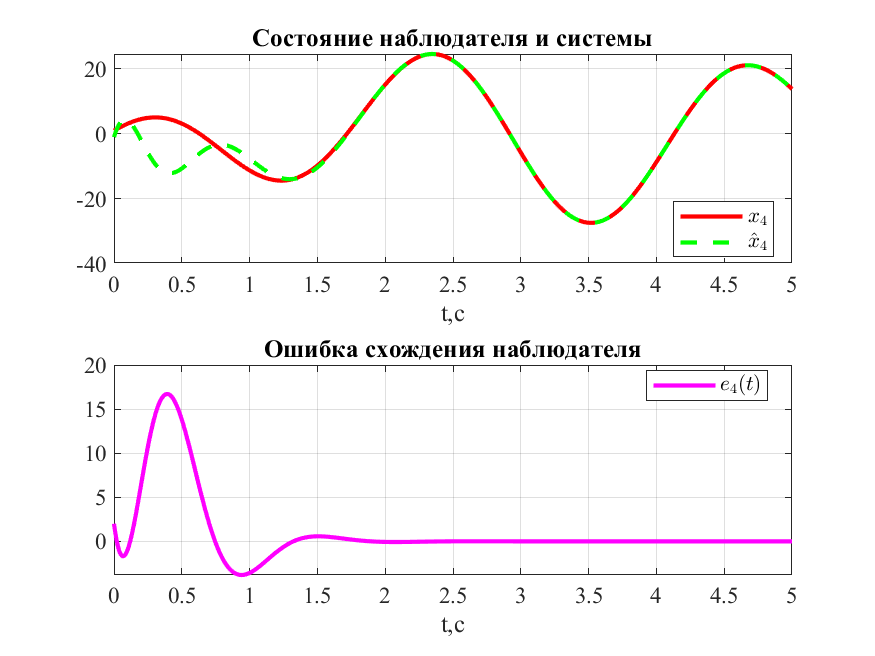
\includegraphics[width=0.8\textwidth]{obsv12.png}
  \caption{Состояние системы и ошибка сходимости}
\end{figure}


\newpage
\subsection{Сравнение выбора собственных чисел для синтеза наблюдателя}
Мы можем заметить, что происходят похожие процессы, как и при синтезе модального регулятора - выбор мод наблюдателя напрямую влияет на характер его схождения к истинной системе.
В первом случае спектр выбран не слишком большим, поэтому матрица коррекции не слишком велика, в итоге мы получили довольно большое перерегулирование (по графику ошибки) при небольшом времени переходного процесса.

Во втором случае мы получили довольно агрессивную сходимость(перерегулирования практически нет, время переходного процесса экстремально мало), но в реальных физических системах вряд ли
наша оценка может так быстро/резки сойтись к истинной безошибочно, 
потому что датчики шумные, и их фильтрация стоит какого-то времени на сбор достаточного количества данных, и последующуб обработку.

В третьем случае наш спектр состоял в том числе и из колебательных мод, поэтому переходный процесс был с перерегулированием куда больше, чем в первом случае, однако время этого процесса стало куда меньше.

\subsection{Вывод}
В этом задании мы работали с полностью наблюдаемой системой, это мы узнали через критерий Калмана.
Мы узнали, что синтезировать наблюдатели можно с разным "характером" сходимости. Для наблюдения мы 
синтезировали модального наблюдателя с помощью уравнения Сильвестра, а также провели серию моделирований с разными наблюдателями, все они показали то, 
что мы сходимся к оригинальной системе с разным качеством переходного процесса - его времени и перерегулирования.
\endinput 
\chapter{Запаздывание}
\label{ch:chap3}

В соответствии с моим вариантом:
$$
    j=2, \tab W_3(s) = \frac{7s+5}{s^2 + 4s}, \tab W_4(s) = \frac{20s^2 +1.6s +2}{10s^3-10s^2-0.1s+0.1}
$$
Необходимо добавить к каждой ПФ звено чистого запаздывания $e^{-\tau s}$.

\section{Передаточная функция $W_3$}

Рассмотрим обновлённую ПФ:
$$
    W_3(s) = \frac{7s+5}{s^2 + 4s}e^{-\tau s}
$$
Получаем её полюса: $\lambda_{1,2} = \{-4, 0\}$, система имеет два устойчивых полюса.

Построим для неё годографы, с разными $\tau$:
\begin{figure}[ht]
    \centering
    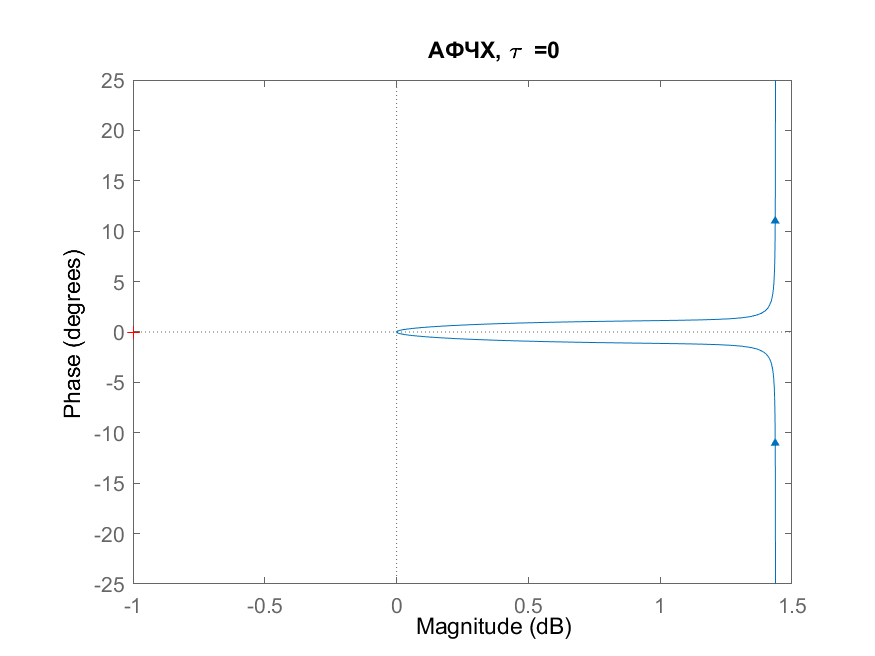
\includegraphics[width=0.7\textwidth]{nyquist_task31_object1.png}
    \caption{Годограф Найквиста для разомкнутой системы, $\tau=0$}
\end{figure}
\newpage
\begin{figure}[ht]
    \centering
    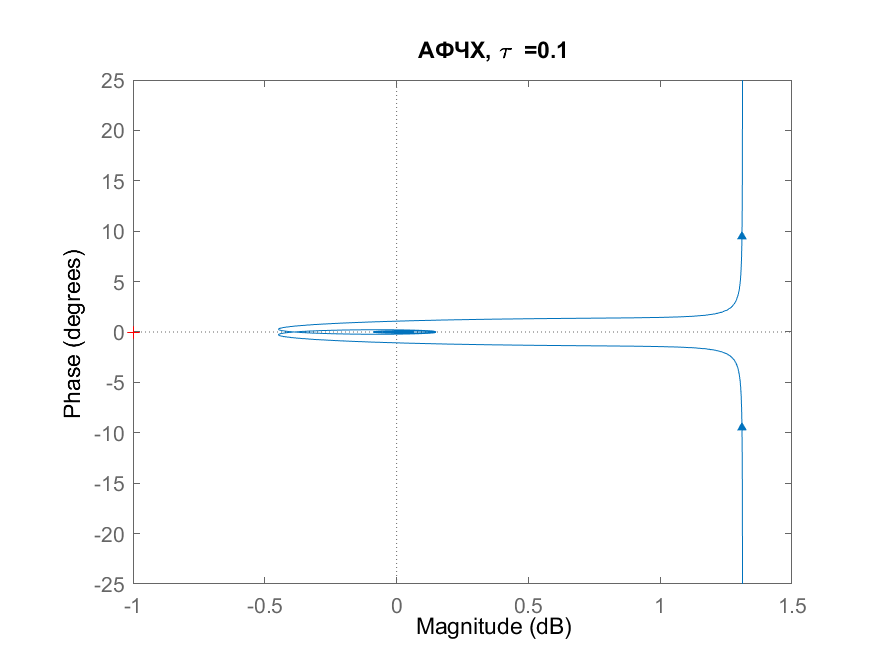
\includegraphics[width=0.7\textwidth]{nyquist_task32_object1.png}
    \caption{Годограф Найквиста для разомкнутой системы, $\tau=0.1$}
\end{figure}
\begin{figure}[ht]
    \centering
    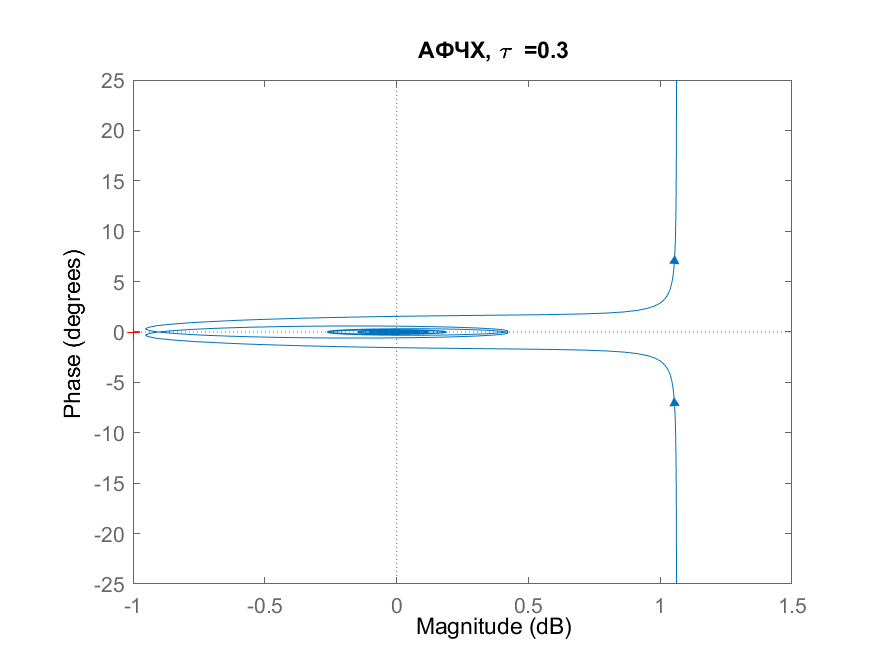
\includegraphics[width=0.7\textwidth]{nyquist_task33_object1.png}
    \caption{Годограф Найквиста для разомкнутой системы, $\tau=0.3$}
\end{figure}
\newpage
\begin{figure}[ht]
    \centering
    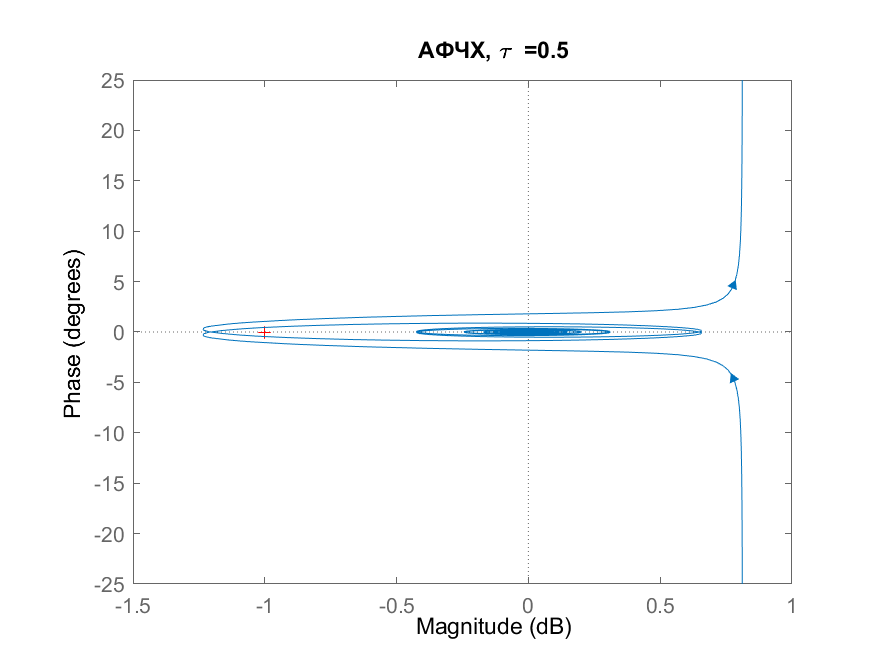
\includegraphics[width=0.7\textwidth]{nyquist_task34_object1.png}
    \caption{Годограф Найквиста для разомкнутой системы, $\tau=0.5$}
\end{figure}
\begin{figure}[ht]
    \centering
    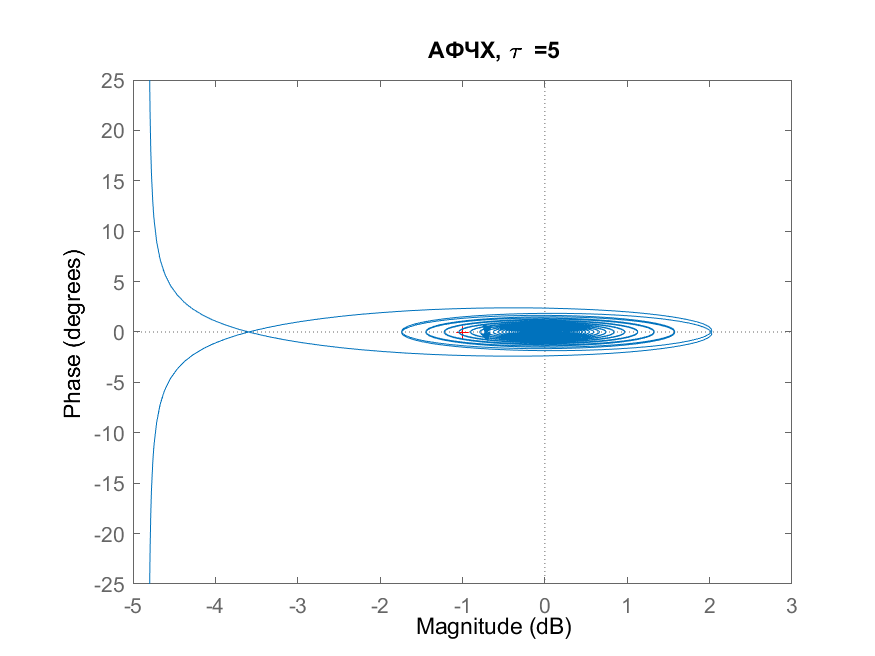
\includegraphics[width=0.7\textwidth]{nyquist_task35_object1.png}
    \caption{Годограф Найквиста для разомкнутой системы, $\tau=5$}
\end{figure}
\newpage
По полученным графикам можно заметить, что замкнутая система будет устойчива примерно до  $\tau< 0.4$, так как до $\tau < 0.3$ ещё всё хорошо и есть небольшой запас коэффицциента запаздывания. После же к системе прибавится два дополнительных неустойчивых полюсов, так как критическая точка попадёт внутрь годографа
и мы получим два оборота по часовой стрелке.

Давайте ниже узнаем точно диапазон - вычислим его аналитически\dots

\newpage
\subsection{Частотные характеристики}
Найдём критическое значение $\tau$. 

\begin{figure}[ht]
    \centering
    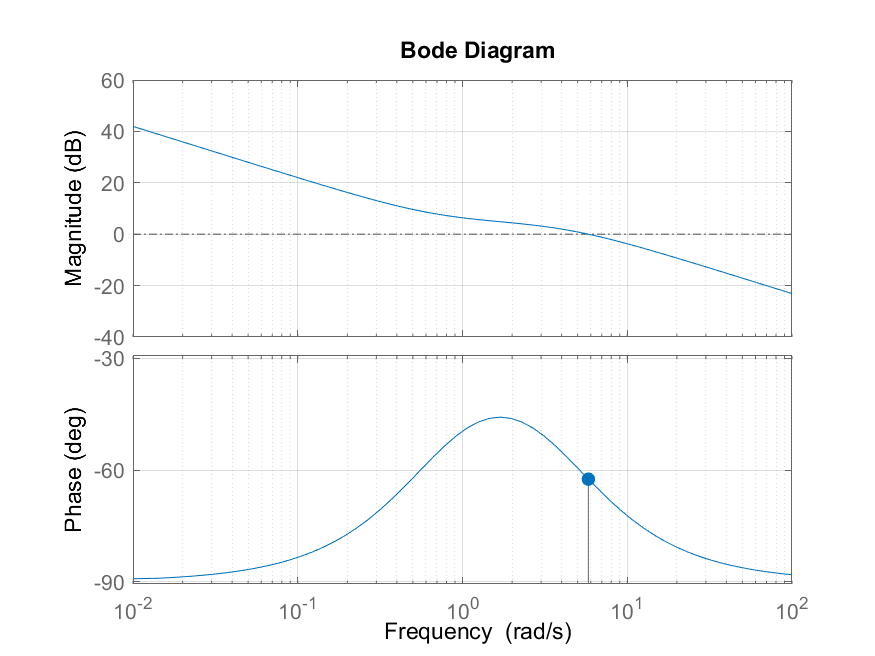
\includegraphics[width=0.7\textwidth]{log_nyquist_task3_object1.png}
    \caption{ЛАФЧХ, $\tau=5.0$}
\end{figure}
С помощью команды $\textrm{allmargin}$ получим информацию о критической точке на графике, её критическое значение и запас по фазе :
$$
 \tau_{crit} \approx 0.35, \tab \phi_3 \approx 117^\circ
$$

Теперь проверим аналитически, посчитаем $\tau_{crit}$, которые мы получили от \textit{matlab} до:
$$
\tau_{max} = \frac{\phi_3}{\omega_\phi}
$$, где $\phi_3$ - запас по фазе, $\omega_\phi$ - частота, соответствующая запасу по фазе. Эти два параметра мы можем найти для двух точек, если приблизим график достаточно точно, тогда получим:
$$
\tau_{crit} = \frac{117.54\pi}{180\cdot 5.8084} = 0.3537
$$

Как можно заметить, аналитически посчитанные совпали с ответами от \textit{allmargin}.


\newpage
\subsection{Переходные функции}
\begin{figure}[ht]
    \centering
    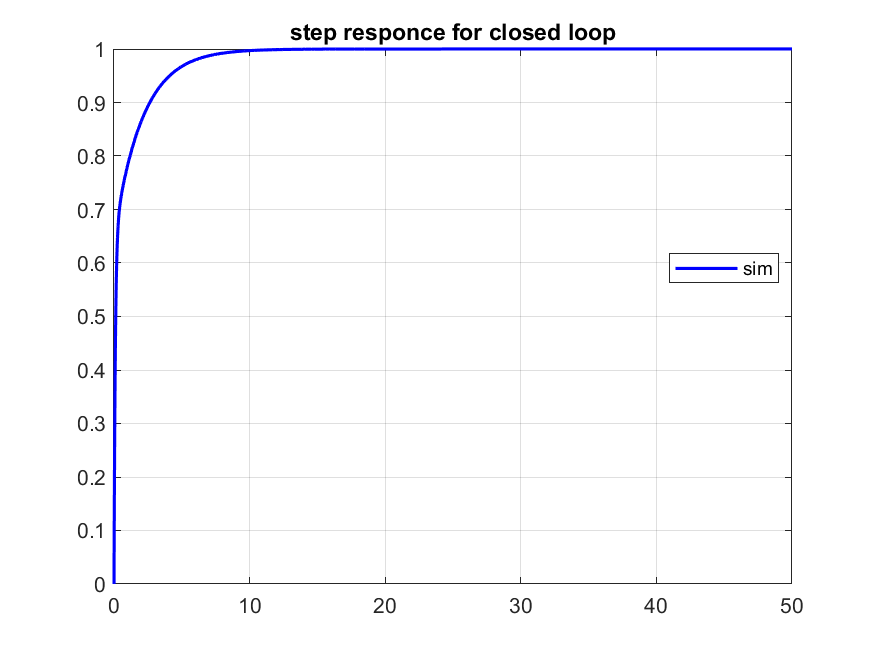
\includegraphics[width=0.7\textwidth]{step_responce31_closed1.png}
    \caption{Переходная функция для замкнутой системы, $\tau=0$}
\end{figure}
\begin{figure}[ht]
    \centering
    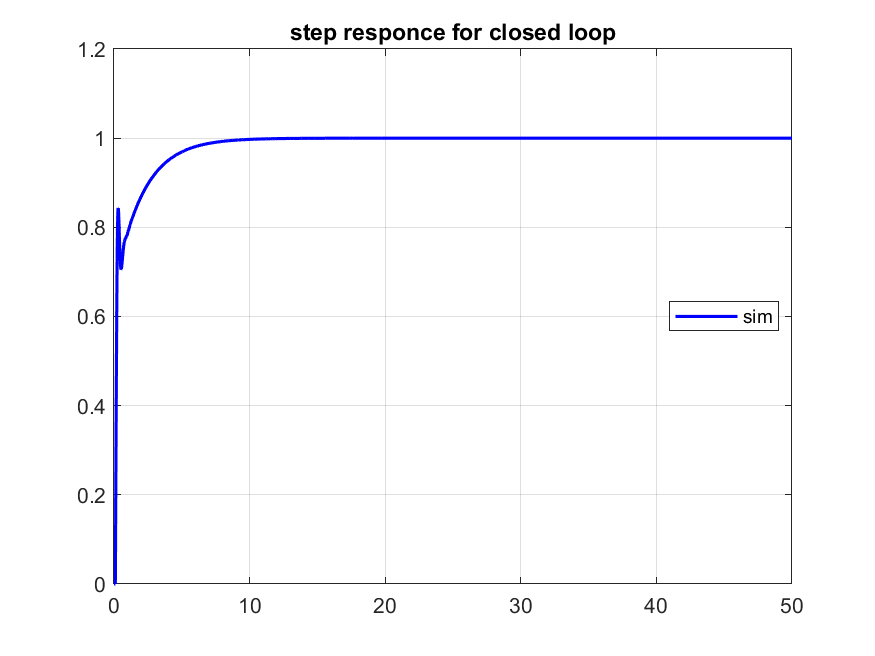
\includegraphics[width=0.7\textwidth]{step_responce32_closed1.png}
    \caption{Переходная функция для замкнутой системы, $\tau=0.1$}
\end{figure}

\newpage
\begin{figure}[ht]
    \centering
    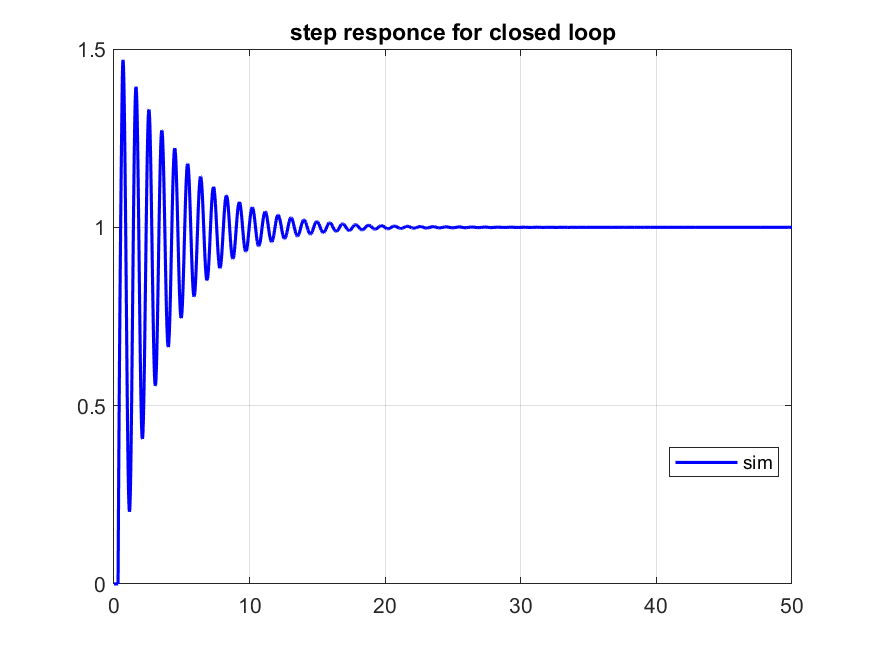
\includegraphics[width=0.7\textwidth]{step_responce33_closed1.png}
    \caption{Переходная функция для замкнутой системы, $\tau=0.3$}
\end{figure}
\begin{figure}[ht]
    \centering
    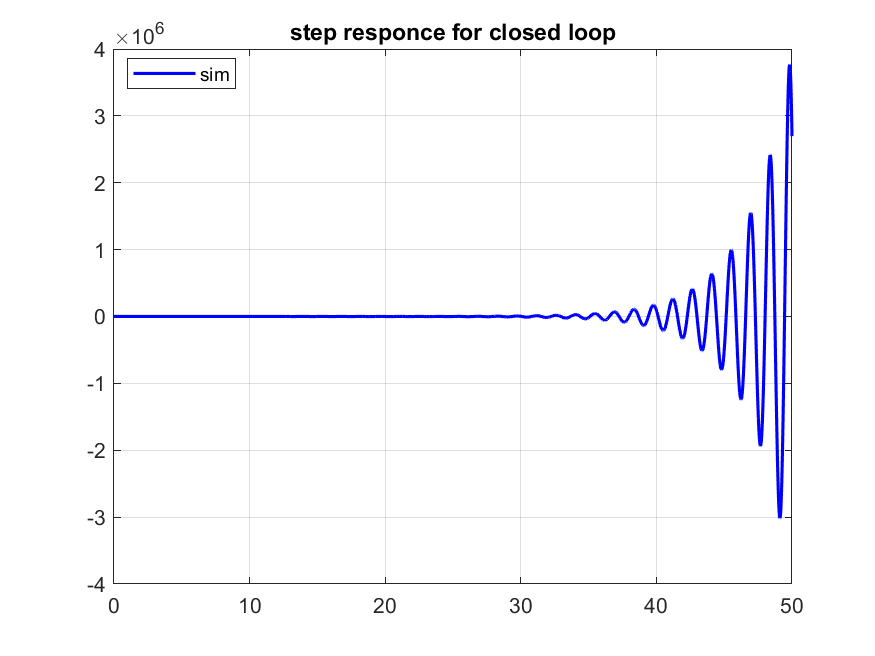
\includegraphics[width=0.7\textwidth]{step_responce34_closed1.png}
    \caption{Переходная функция для замкнутой системы, $\tau=0.5$}
\end{figure}
\newpage
\begin{figure}[ht]
    \centering
    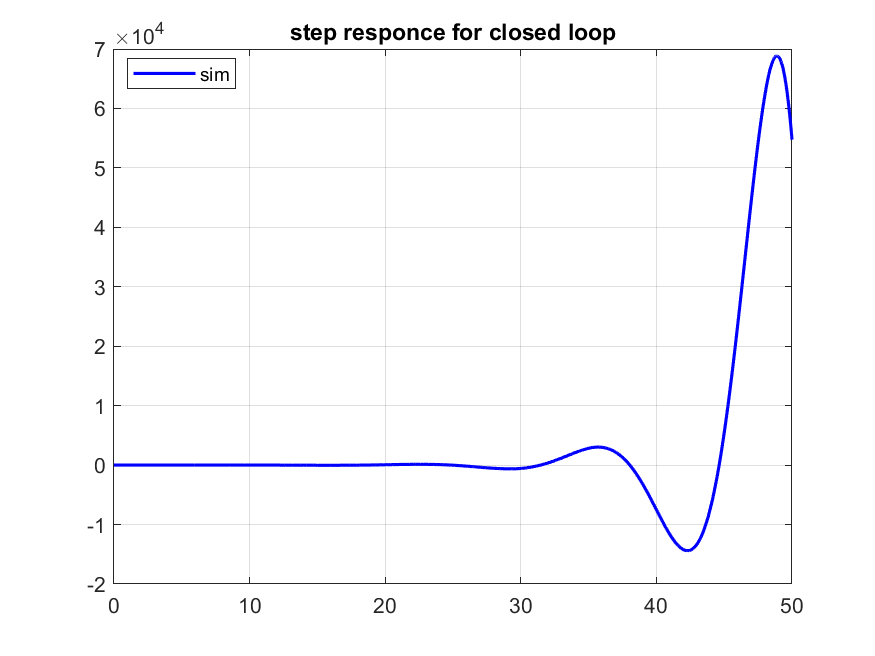
\includegraphics[width=0.7\textwidth]{step_responce35_closed1.png}
    \caption{Переходная функция для замкнутой системы, $\tau=5$}
\end{figure}
По графикам можно заметить, что аналитические выкладки подтвердились - замкнутая система устойчива будет устойчива лишь при $\tau < 0.35 $.


\section{Передаточная функция $W_4$}
Рассмотрим обновлённую ПФ:
$$
    W_4(s) = \frac{20s^2 +1.6s +2}{10s^3-10s^2-0.1s+0.1}e^{-\tau s}
$$
Получим её полюса: $\lambda_{1,2,3} \approx \{-0.23, 0.11 \pm 0.17j \}$, система имеет два неустойчивых и один устойчивых полюс.

Построим для неё годографы, с разными $\tau$:
\begin{figure}[ht]
    \centering
    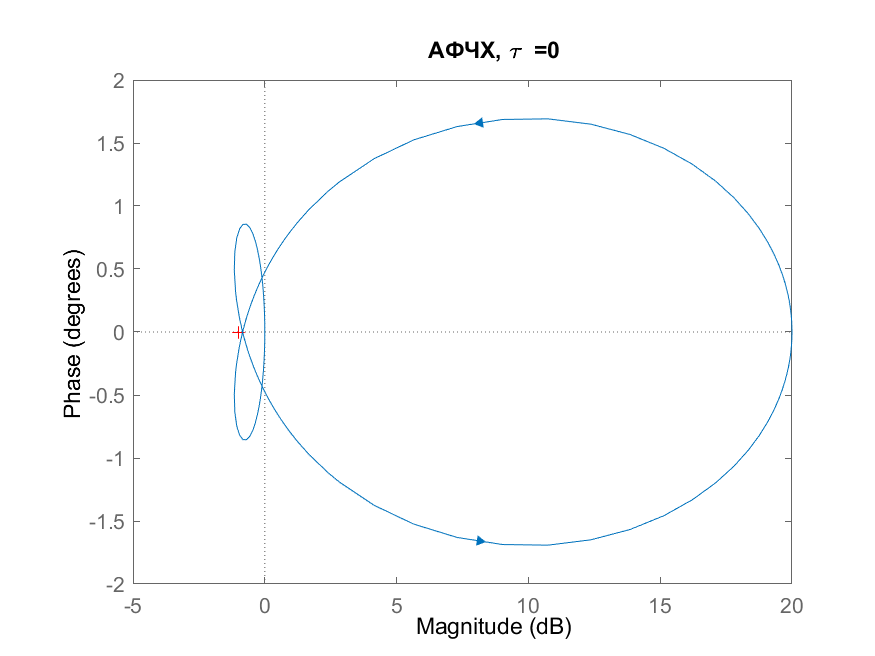
\includegraphics[width=0.7\textwidth]{nyquist_task31_object2.png}
    \caption{Годограф Найквиста для разомкнутой системы, $\tau=0$}
\end{figure}
\newpage
\begin{figure}[ht]
    \centering
    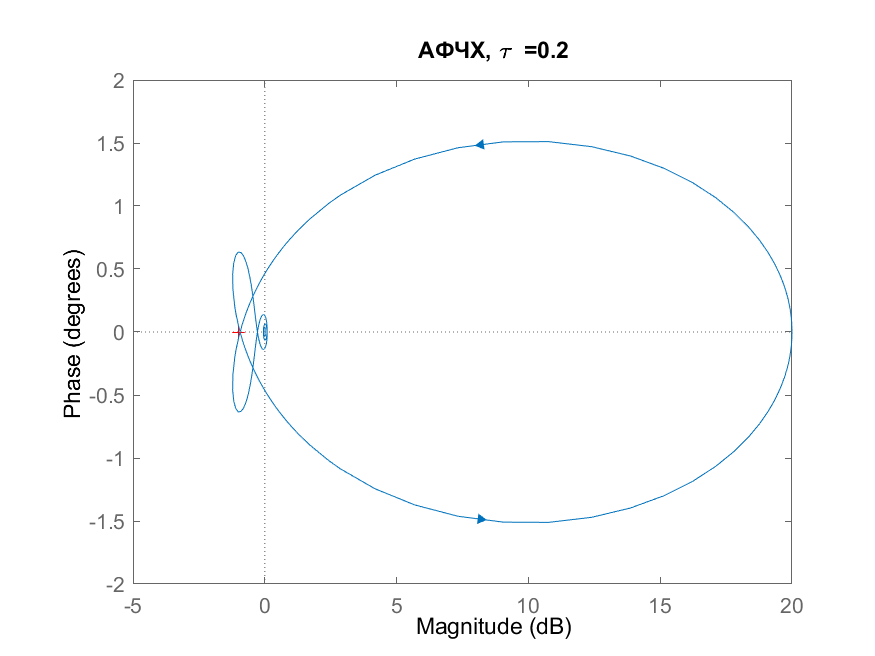
\includegraphics[width=0.7\textwidth]{nyquist_task33_object2.png}
    \caption{Годограф Найквиста для разомкнутой системы, $\tau=0.2$}
\end{figure}

\begin{figure}[ht]
    \centering
    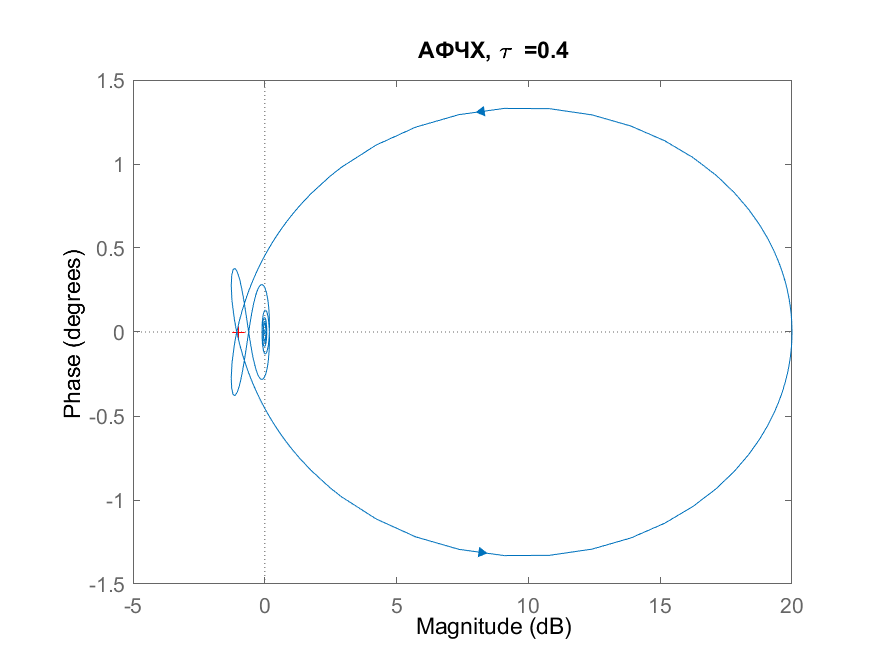
\includegraphics[width=0.7\textwidth]{nyquist_task35_object2.png}
    \caption{Годограф Найквиста для разомкнутой системы, $\tau=0.4$}
\end{figure}
\newpage
\begin{figure}[ht]
    \centering
    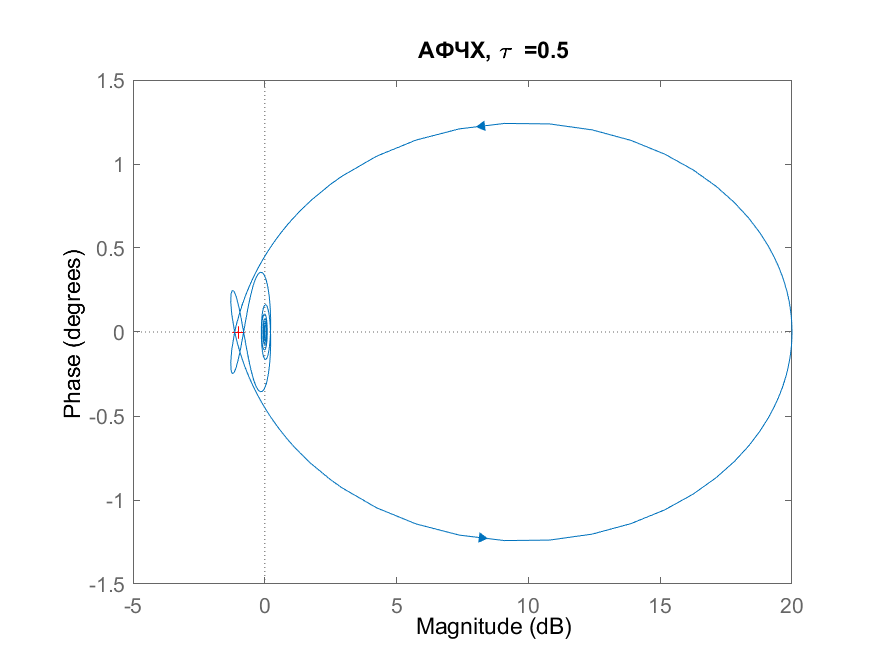
\includegraphics[width=0.7\textwidth]{nyquist_task36_object2.png}
    \caption{Годограф Найквиста для разомкнутой системы, $\tau=0.5$}
\end{figure}
\begin{figure}[ht]
    \centering
    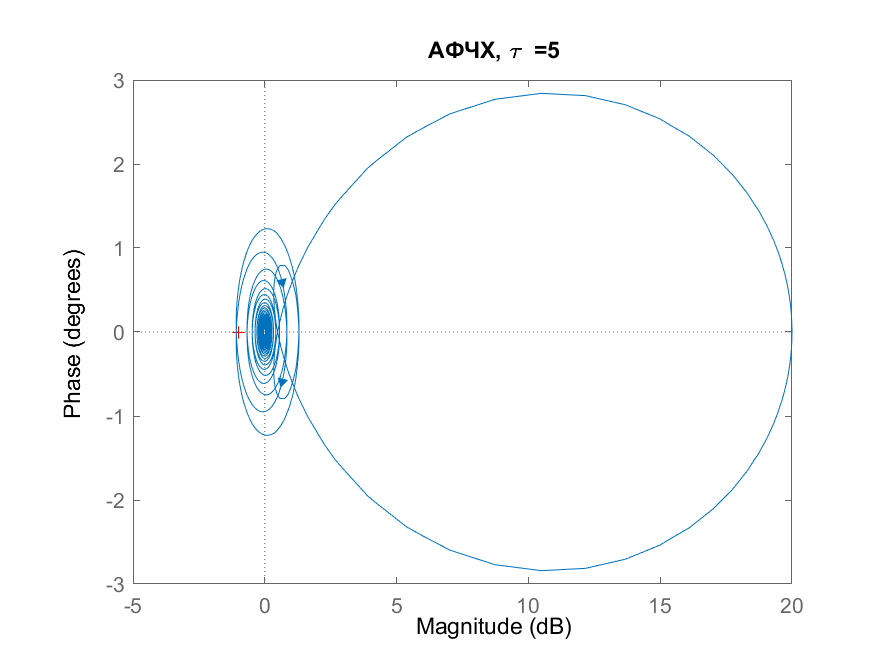
\includegraphics[width=0.7\textwidth]{nyquist_task39_object2.png}
    \caption{Годограф Найквиста для разомкнутой системы, $\tau=5$}
\end{figure}
\newpage
\begin{figure}[ht]
    \centering
    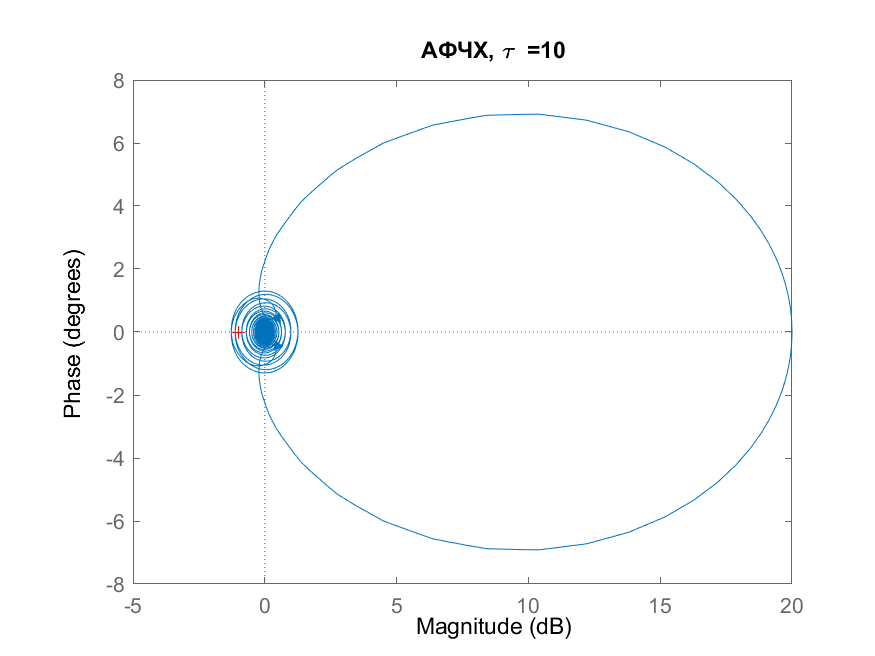
\includegraphics[width=0.7\textwidth]{nyquist_task310_object2.png}
    \caption{Годограф Найквиста для разомкнутой системы, $\tau=10$}
\end{figure}
По полученным графикам пока рано говорить об устойчивости в зависимости от задержки, потому что, например, примерно до $\tau< 0.3$ мы не получаем обороты, которые могут убрать нам неустойчивые полюса, а могут и прибавить, зависит от направления оборотов.
После же, при $\tau > 0.3$ пока рано о чём-либо заявлять, количество и направления трудно установить, поэтому лучше рассмотреть логарифмический критерий Найквиста и аналитически установить диапазон для $\tau$\dots

\newpage
\subsection{Частотные характеристики}
Попробуем найти критическое значение $\tau$. 

\begin{figure}[ht]
    \centering
    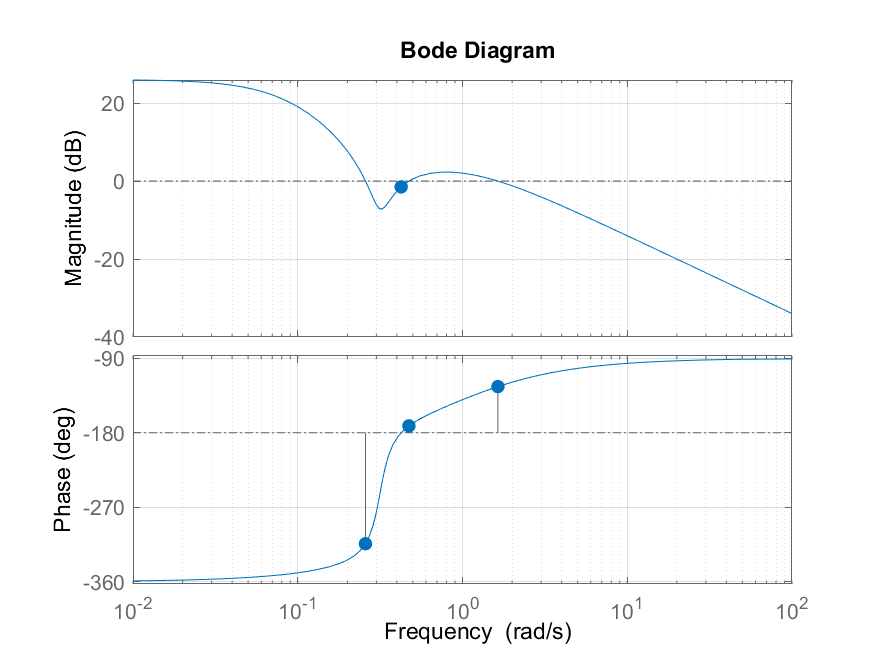
\includegraphics[width=0.7\textwidth]{log_nyquist_task3_object2.png}
    \caption{ЛАФЧХ, $\tau=5.0$}
\end{figure}

Однако всё же с помощью функции \textit{allmargin}  мы можем получить критическое допустимое время запаздывания и запас по фазе для этих точек:


$$
\begin{aligned}
    \tau_{crit1}=15.2, \tab \phi_{13}=-135^\circ, \\   
    \tau_{crit2}=0.3, \tab \phi_{23}=5.5^\circ, \\
    \tau_{crit3}=0.59, \tab \phi_{33}=46^\circ
\end{aligned}
$$

% Как можно заметить их будет три, но при проверке критерия можно заметить:
% нам нужно, чтобы сумма положительных и отриательных переходов через критический отрезок была равна $\frac{r}{2}= 1$. Но при $L(\omega) > 0$ у нас нет переходов, поэтому замкнутая система будет нейстойчивой. У системы не будет запаса устойчивости по фазе.

Как можно заметить, один из кандидатов на запас по фазе у нас отрицательный, поэтому его отбросим и сосредоточимся на двух оставшихся критических точках.

Давайте аналитически посчитаем $\tau_{crit2}, \tau_{crit3}$, которые мы получили от \textit{matlab} до:
$$
\tau_{max} = \frac{\phi_3}{\omega_\phi}
$$, где $\phi_3$ - запас по фазе, $\omega_\phi$ - частота, соответствующая запасу по фазе. Эти два параметра мы можем найти для двух точек, если приблизим график достаточно точно, тогда получим:
$$
\tau_{crit2} = \frac{8.26\pi}{180\cdot 0.4727} \approx 0.304 , \tab \tau_{crit3} = \frac{55.72\pi}{180\cdot 1.6401} \approx 0.59
$$
Получается, что замкнутая система устойчива будет устойчива в диапазоне между двумя критическими значениями, то есть: $\tau \in (0.304; 0.59)$.
Как можно заметить, аналитически посчитанные совпали с ответами от \textit{allmargin}. Проверим это на практике:

\newpage
\subsection{Переходные функции}
\begin{figure}[ht]
    \centering
    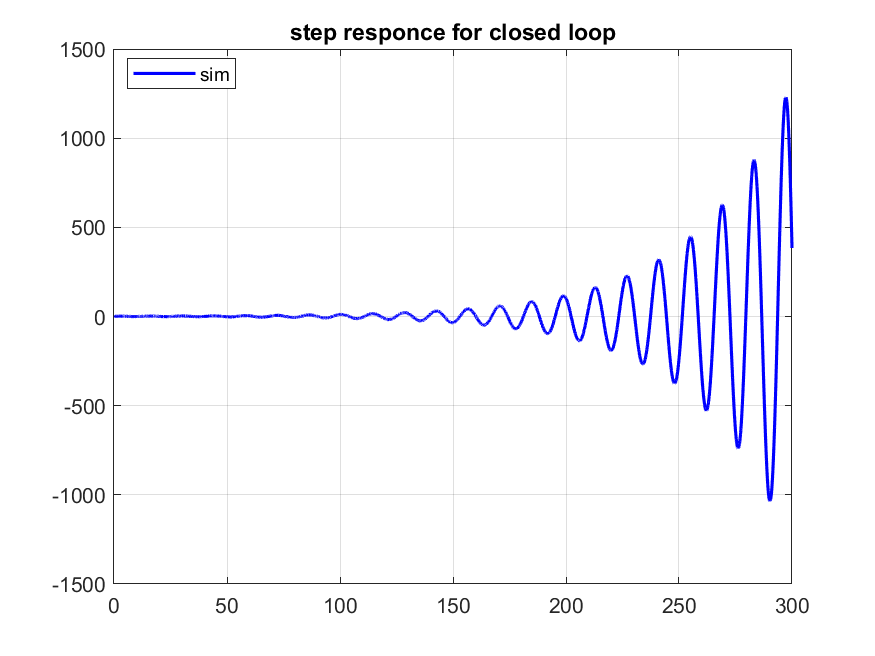
\includegraphics[width=0.7\textwidth]{step_responce31_closed2.png}
    \caption{Переходная функция для замкнутой системы, $\tau=0$}
\end{figure}
\begin{figure}[ht]
    \centering
    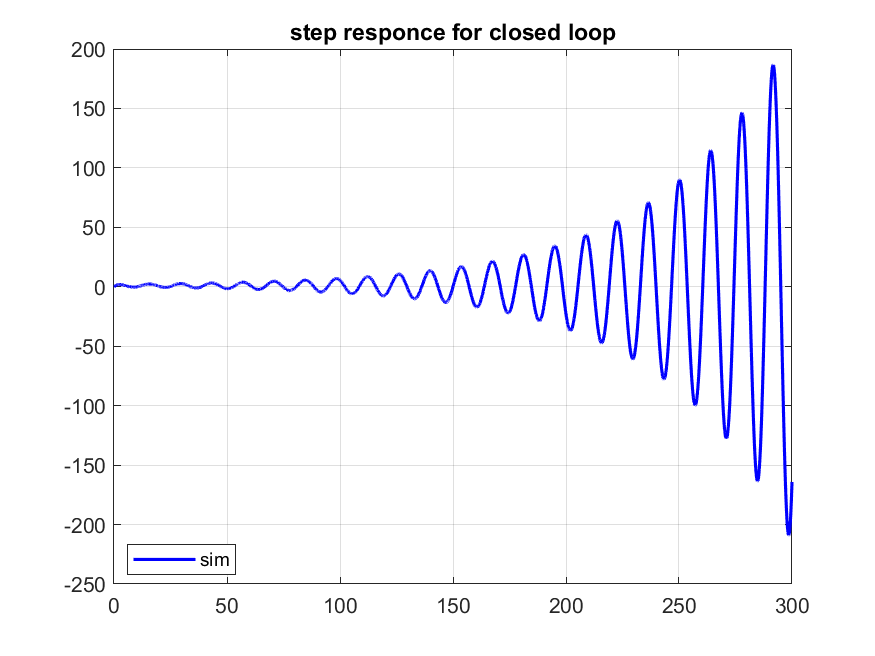
\includegraphics[width=0.7\textwidth]{step_responce32_closed2.png}
    \caption{Переходная функция для замкнутой системы, $\tau=0.1$}
\end{figure}

\newpage
\begin{figure}[ht]
    \centering
    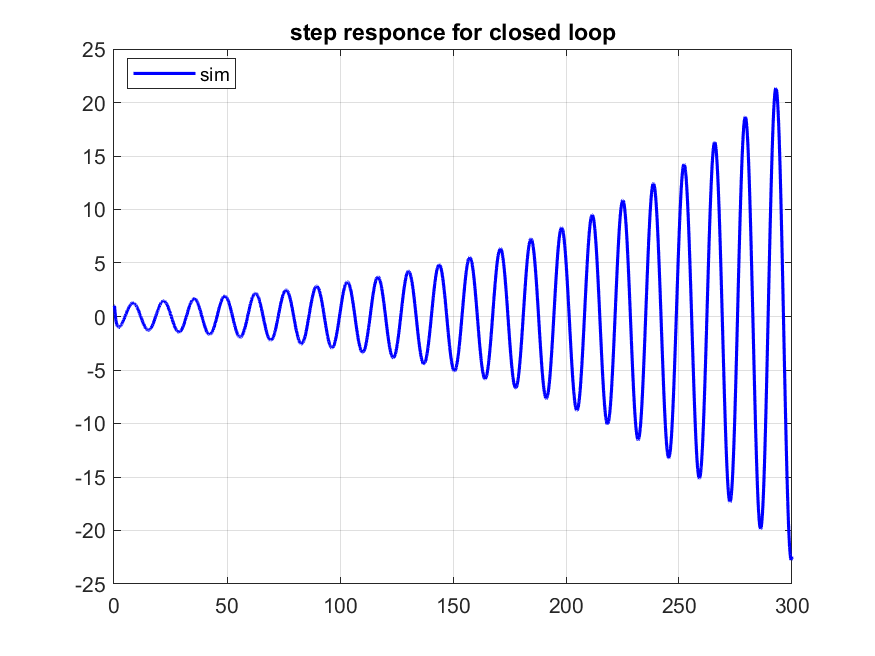
\includegraphics[width=0.7\textwidth]{step_responce33_closed2.png}
    \caption{Переходная функция для замкнутой системы, $\tau=0.2$}
\end{figure}
\begin{figure}[ht]
    \centering
    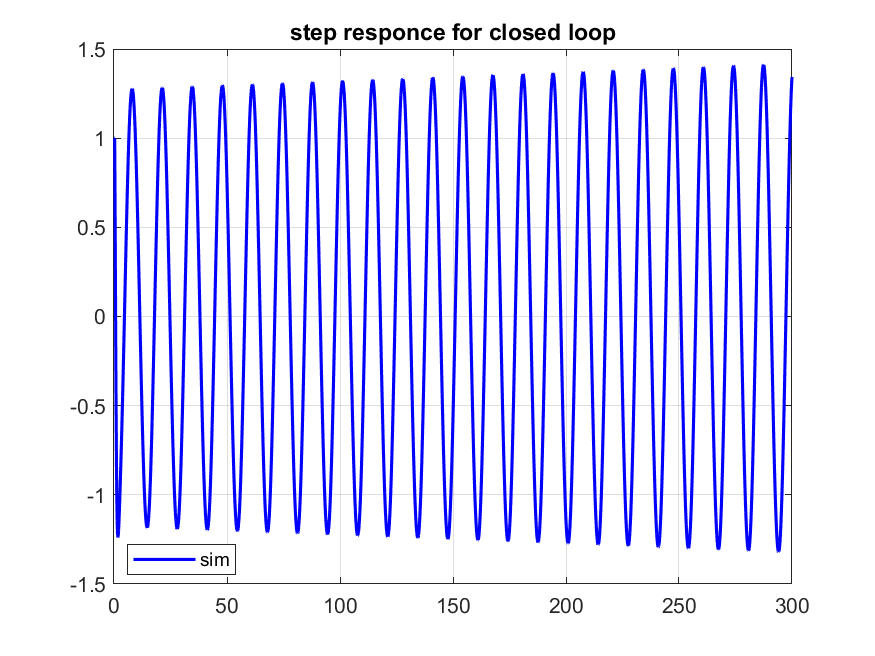
\includegraphics[width=0.7\textwidth]{step_responce34_closed2.png}
    \caption{Переходная функция для замкнутой системы, $\tau=0.3$}
\end{figure}

\newpage
\begin{figure}[ht]
    \centering
    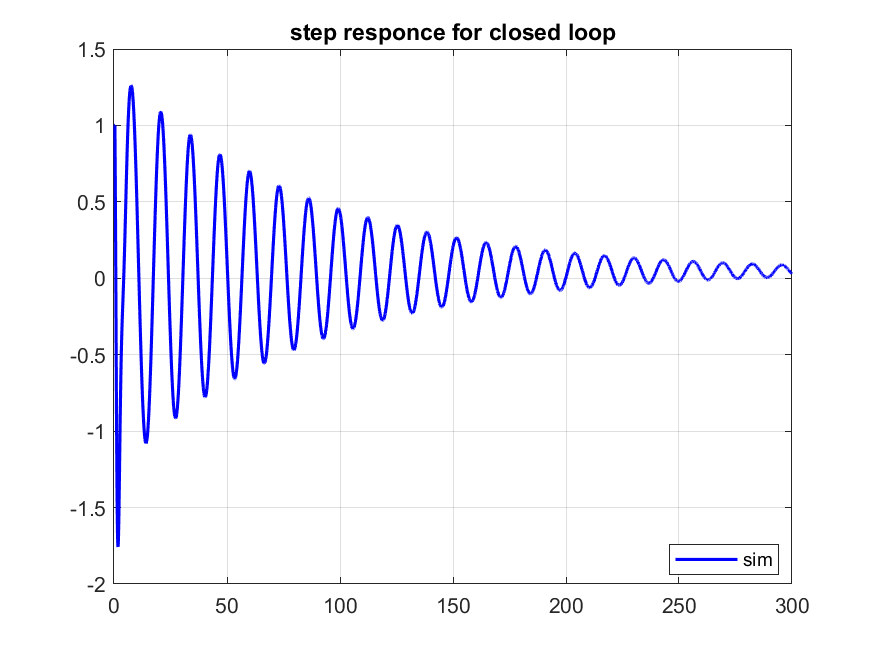
\includegraphics[width=0.7\textwidth]{step_responce35_closed2.png}
    \caption{Переходная функция для замкнутой системы, $\tau=0.4$}
\end{figure}
\begin{figure}[ht]
    \centering
    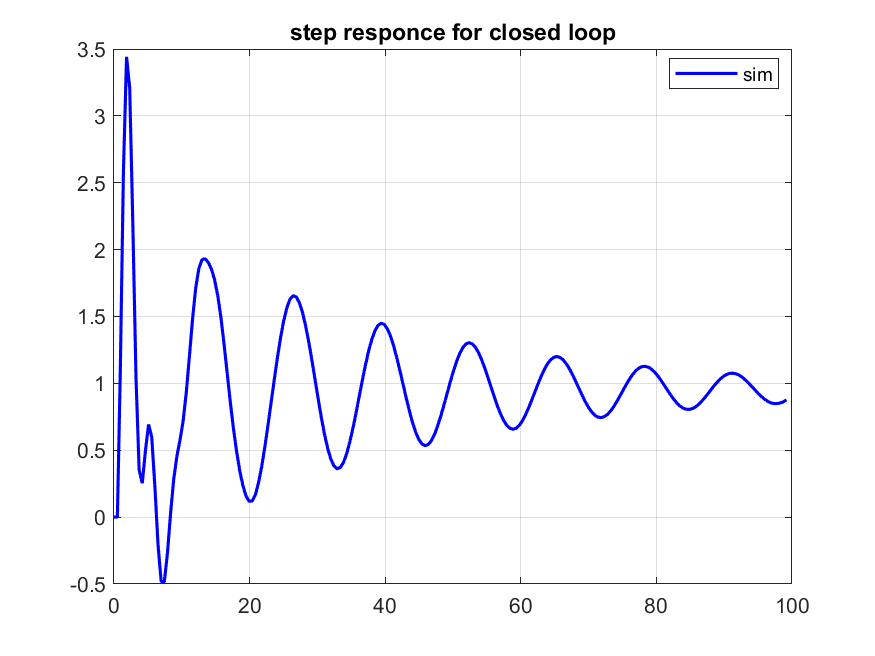
\includegraphics[width=0.7\textwidth]{step_responce36_closed2.png}
    \caption{Переходная функция для замкнутой системы, $\tau=0.5$}
\end{figure}

\newpage
\begin{figure}[ht]
    \centering
    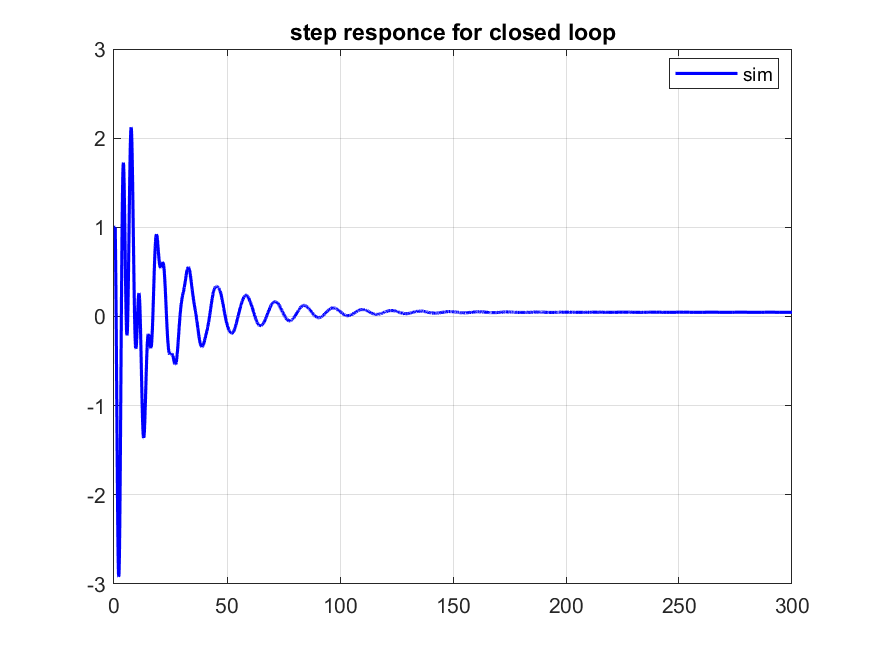
\includegraphics[width=0.7\textwidth]{step_responce37_closed2.png}
    \caption{Переходная функция для замкнутой системы, $\tau=0.55$}
\end{figure}
\begin{figure}[ht]
    \centering
    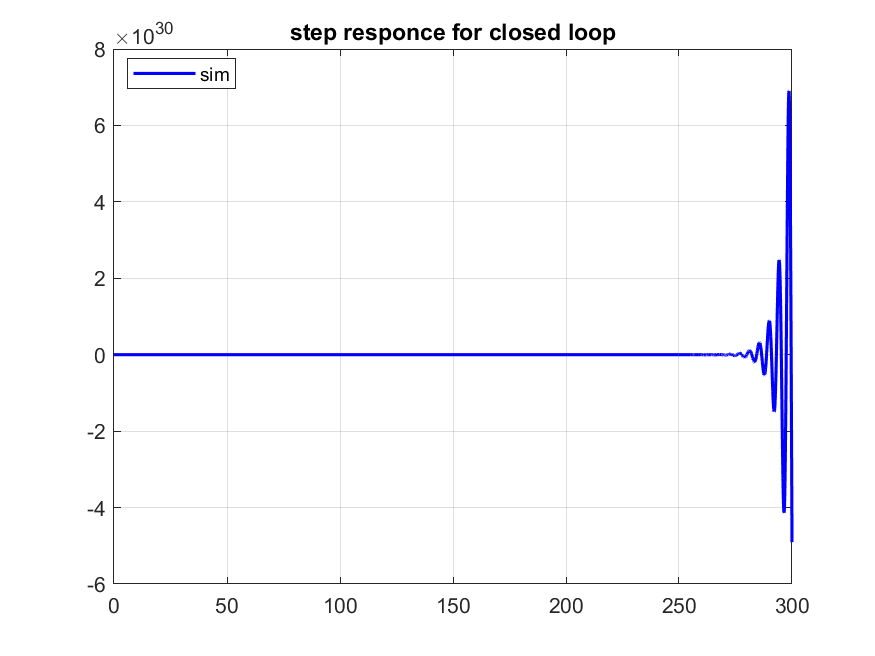
\includegraphics[width=0.7\textwidth]{step_responce38_closed2.png}
    \caption{Переходная функция для замкнутой системы, $\tau=0.7$}
\end{figure}

\newpage
\begin{figure}[ht]
    \centering
    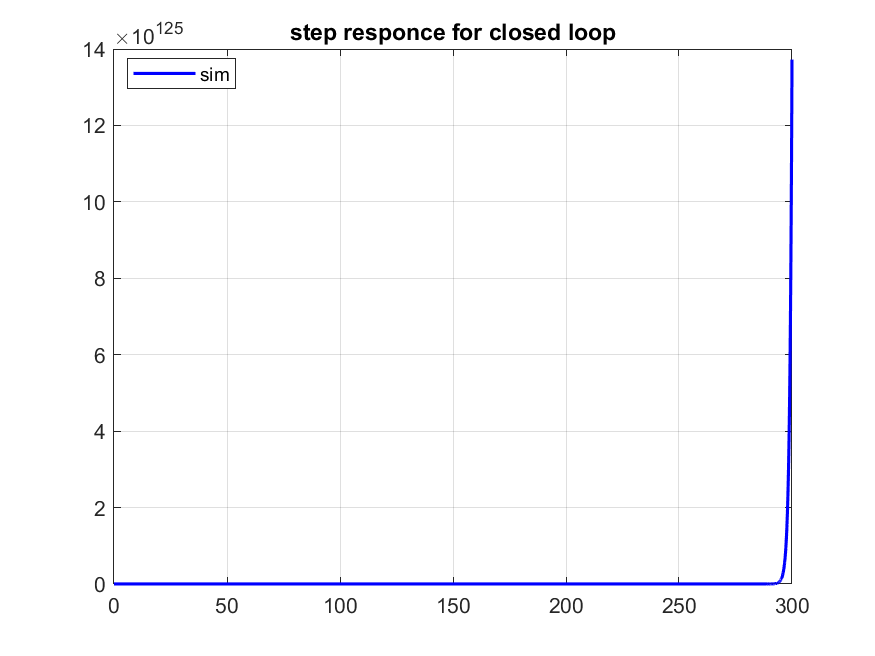
\includegraphics[width=0.7\textwidth]{step_responce39_closed2.png}
    \caption{Переходная функция для замкнутой системы, $\tau=5$}
\end{figure}
\begin{figure}[ht]
    \centering
    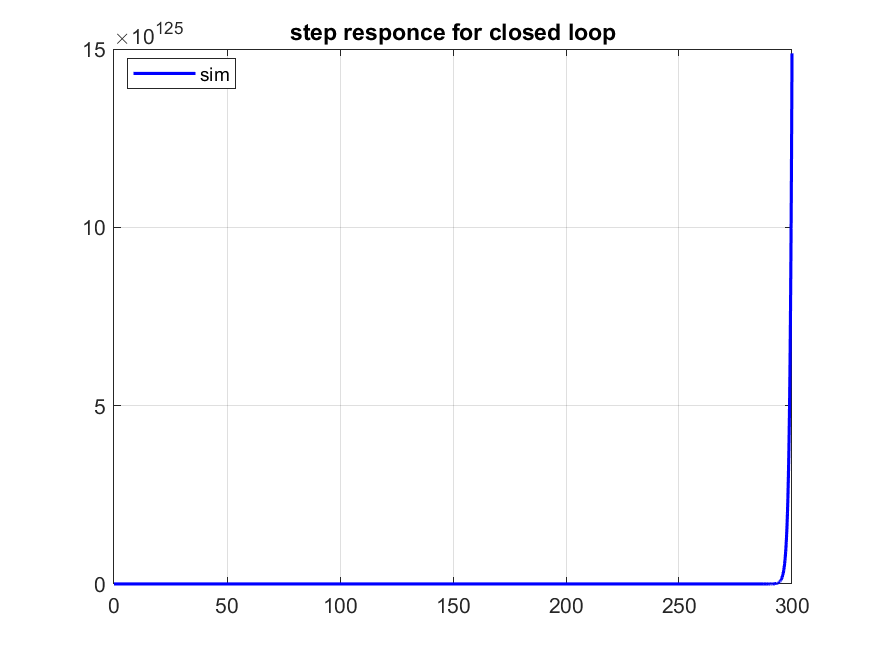
\includegraphics[width=0.7\textwidth]{step_responce310_closed2.png}
    \caption{Переходная функция для замкнутой системы, $\tau=10$}
\end{figure}

По графикам можно заметить, что аналитические выкладки подтвердились - замкнутая система устойчива будет устойчива при $\tau \in (0.304; 0.59)$.

\endinput
\chapter{Пружинка}
\label{ch:chap4}
Параметры системы:
$$
M = 24, \tab k = 112
$$
Даны уравнения пружинного маятника:
$$
F_{ela} = -kx, \tab F = ma = m\ddot{x}
$$
Входом считается $F_{ext}(t)$ - некая внешняя соосно направленная сила, а $x(t)$ - выход. 
Запишем второй закон Ньютона, чтобы объединить уравнения:
$$
    F = F_{ela} + F_{ext} = m\ddot{x}
$$

\section{Передаточная функция}
Перейдем в операторную форму Лапласа:
$$
 -kX + F_{ext} = ms^2X
$$
$$
W(s) = \frac{1}{ms^2 + k}
$$
По отсутствию компоненты $s$ в знаменателе видно, что это - \textit{консервативное звено}, его общий вид:
$$
W(S) = \frac{K}{T^2s^2 + 1}
$$ Тогда в нашем случае $K = \frac{1}{mk} \approx 4\cdot 10^{-4}$ и $T = \sqrt{\frac{1}{k}} \approx 0.09$
\section{Временные  характеристики}
$$
\begin{aligned}
    y_{i.r.}(t) = \mathcal{L}^{-1}\{\frac{K}{T^2s^2 + 1}\} = \mathcal{L}^{-1}\{\frac{K}{T^2(s^2 + \frac{1}{T^2})}\} = \mathcal{L}^{-1}\{\frac{K \frac{1}{T}}{\frac{1}{T}T^2(s^2 + \frac{1}{T^2})}\} = \\
    \frac{K}{T} sin(\frac{1}{T}t)
\end{aligned}
$$
$$
    \begin{aligned}
        y_{s.r.}(t) = \mathcal{L}^{-1}\{\frac{K}{s(T^2s^2 + 1)}\} = \mathcal{L}^{-1}\{\frac{K}{s} - \frac{T^2s}{T^2s^2 + 1}\} = \mathcal{L}^{-1}\{\frac{K}{s} - \frac{Ks}{s^2 + \frac{1}{T^2}}\} = \\
        K - K\cdot cos(\frac{1}{T}t)
    \end{aligned}
$$
\newpage
\begin{figure}[ht]
  \centering
  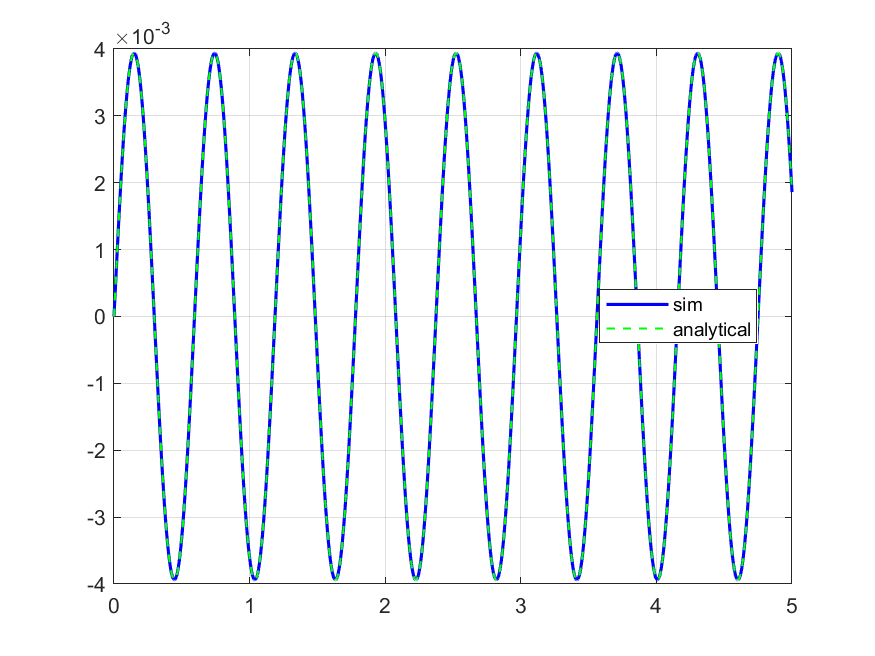
\includegraphics[width=0.8\textwidth]{impulse_responce4.png}
  \caption{Воздействие - \textrm{impulse responce}}
\end{figure}

\begin{figure}[ht]
    \centering
    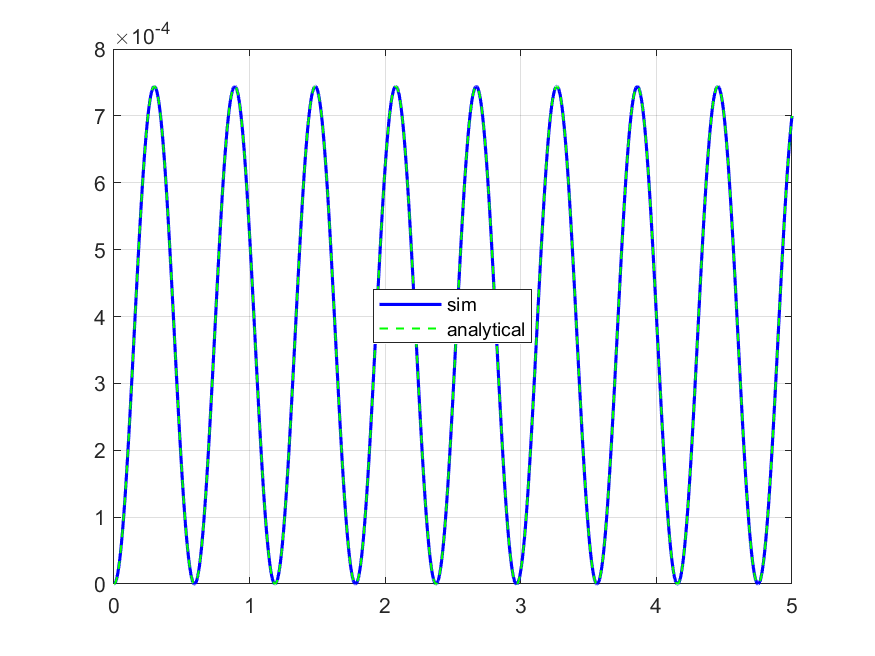
\includegraphics[width=0.8\textwidth]{step_responce4.png}
    \caption{Воздействие - \textrm{step responce}}
  \end{figure}
\newpage
\section{Частотные характеристики}
$$
W(j\omega) =  \frac{K}{T^2(j\omega)^2 + 1} = \frac{K}{1  - T^2\omega^2} + 0
$$
Амплитудно-частотная характеристика:
$$
A(\omega) = \sqrt{P^2 + Q^2} = \sqrt{(\frac{K}{1  - T^2\omega^2})^2 + 0^2} =  \frac{K}{|1  - T^2\omega^2|}
$$
Логарифмическая-Амплитудно-частотная характеристика:
$$
L(\omega) = 20lg(A) = 20lg(K) - 20lg(|1  - T^2\omega^2|)
$$
Фазовая-частотная характеристика:
$$
\phi(\omega) = -atan2(0, \frac{K}{1  - T^2\omega^2})
$$
\newpage
\begin{figure}[ht]
  \centering
  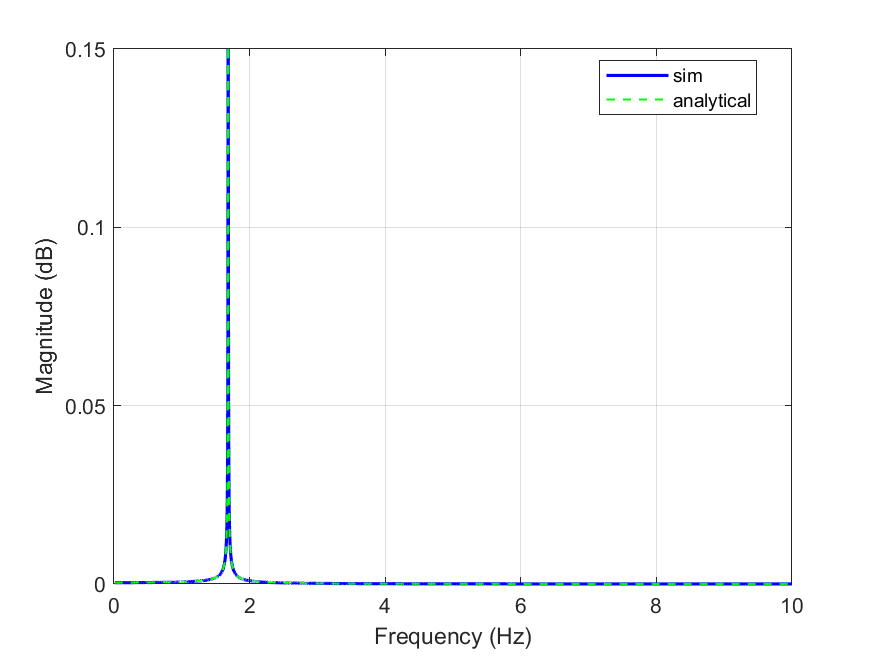
\includegraphics[width=0.8\textwidth]{freq_ampl4.png}
\caption{Сравнение - АЧХ}
\end{figure}

\begin{figure}[ht]
    \centering
    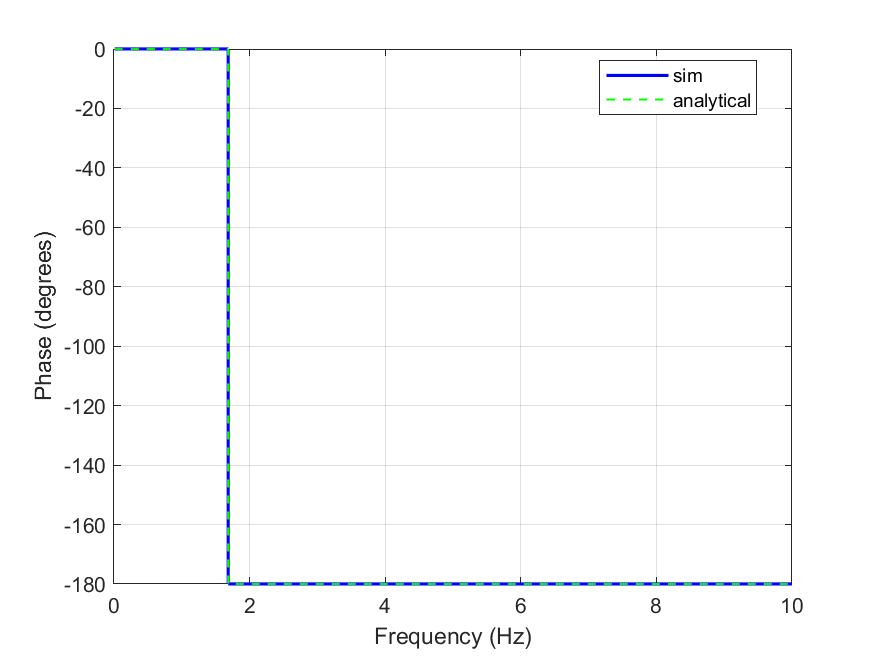
\includegraphics[width=0.8\textwidth]{freq_phase4.png}
  \caption{Сравнение - ФЧХ}
  \end{figure}
\newpage
\begin{figure}[ht]
    \centering
    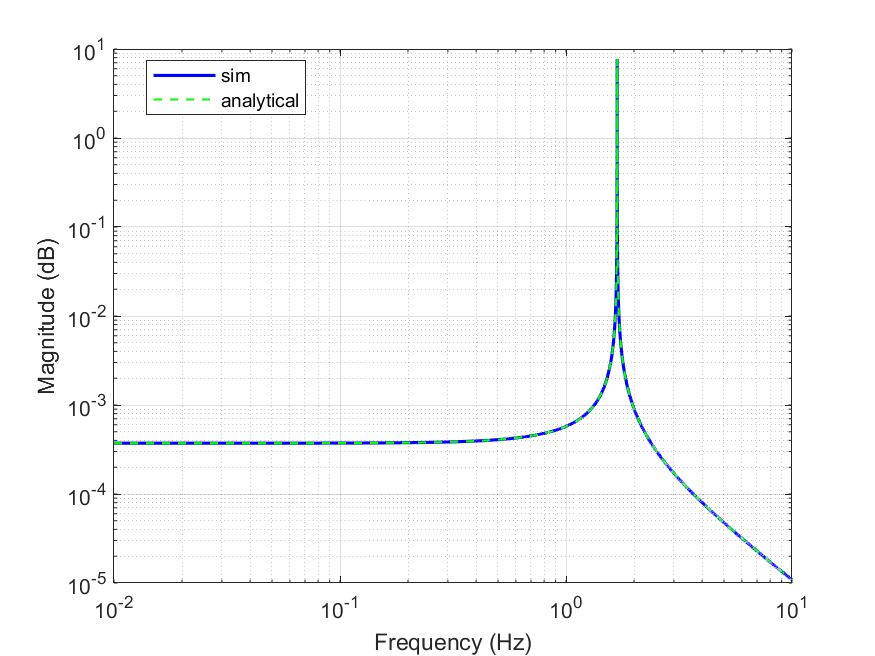
\includegraphics[width=0.8\textwidth]{lfreq_ampl4.png}
  \caption{Сравнение - ЛАЧХ}
  \end{figure}
  
  \begin{figure}[ht]
      \centering
      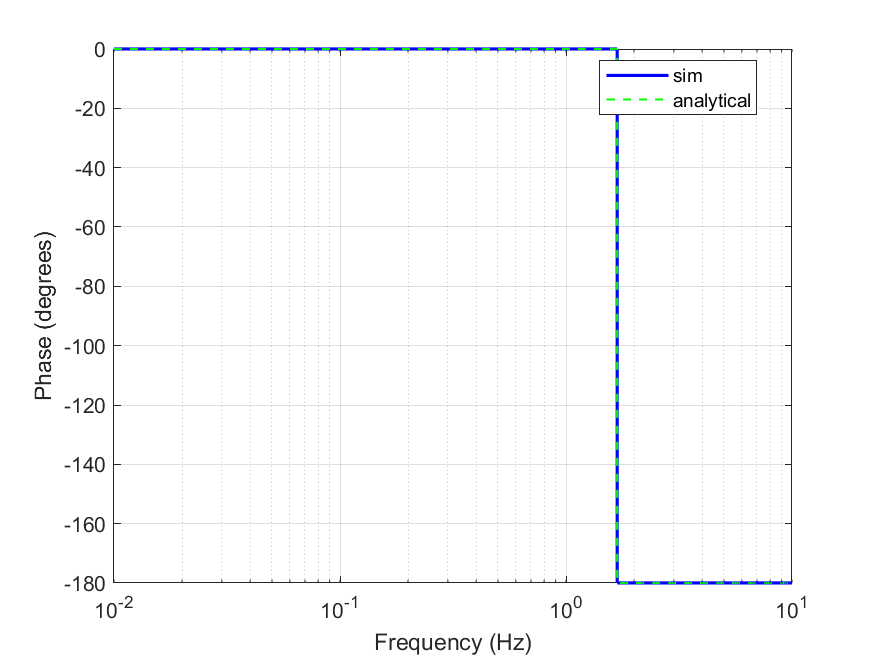
\includegraphics[width=0.8\textwidth]{lfreq_phase4.png}
    \caption{Сравнение - ЛФЧХ}
    \end{figure}

    % \begin{figure}[ht]
    %   \centering
    %   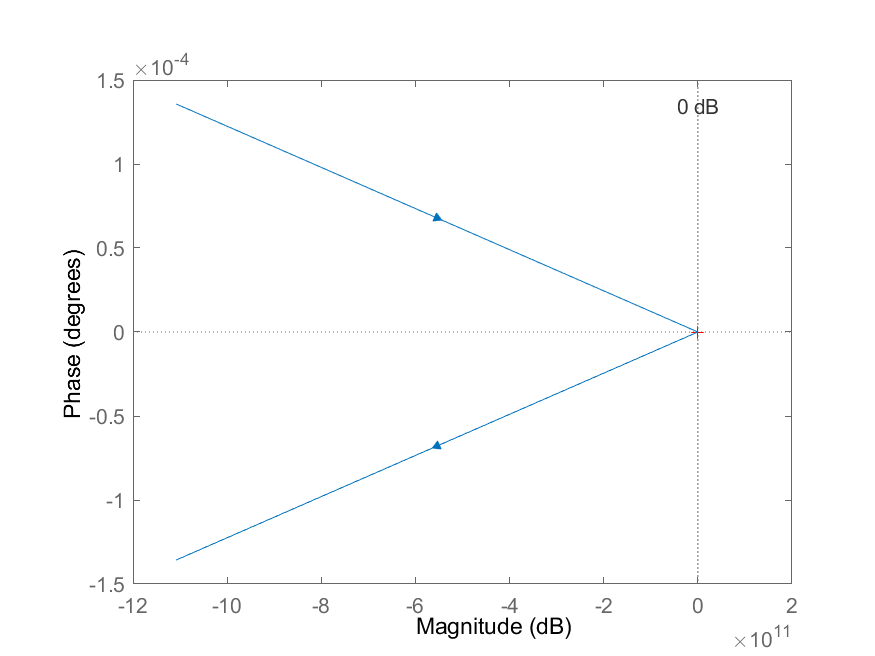
\includegraphics[width=0.8\textwidth]{nyquist4.png}
    % \caption{АФЧХ}
    % \end{figure}
\newpage

\endinput
\chapter{Исследование управляемости по выходу}
\label{ch:chap5}
\section{Условие задачи}

Необходимо рассмотреть систему:
$$
  \begin{cases}
    \dot{x} = Ax + Bu \\
    y = Cx + Du
  \end{cases}
$$ и выполнить следующие шаги:

\begin{itemize}
    \item Найти Жорданову (или диагональную) форму системы.
    \item Определить управляемость и наблюдаемость каждого из собственных чисел и системы в целом.
    \item Найти матрицу управляемости системы по выходу при $D = \mathbf{0}_{2×2}$, определить её
    ранг, сделать вывод об управляемости системы по выходу.
    \item Проанализировав полученные результаты, попытаться сделать выводы о причинах 
    управляемости или неуправляемости системы по выходу.
    \item Предложить такую матрицу cвязи $D$, которая могла бы обеспечить 
    полную управляемость по выходу.
\end{itemize}

\section{Решение задачи}

Параметры для объекта:
$$
  A = \begin{bmatrix}
  3 & -6 & 4 \\
  4 & -5 & 4 \\
  -4 & 4 & -5 
  \end{bmatrix} \tab
  B = \begin{bmatrix}
    -1 \\ 3 \\ 1 
  \end{bmatrix} \tab
  C = \begin{bmatrix}
    0 & -4 & -3 \\
    0 & -8 & -6
  \end{bmatrix}
$$

\subsection{Исследование управляемости и наблюдаемости системы}


Найдём Жорданову форму системы, в общем виде она выглядит следующим образом:
$$
    \begin{cases}
      \dot{\hat{x}} = P^{-1}\boldsymbol{A}P \hat{x} + P^{-1}\boldsymbol{B} u \\
      y = \boldsymbol{C}P\hat{x} + Du
    \end{cases}
$$
В нашем случае жорданова клетка и входное/выходное воздействие таково:
$$
    \mathbf{A} = \begin{bmatrix}
        -1 & 0 & 0 \\
        0 & -3 & -2 \\
        0 & 2 & -3 
        \end{bmatrix} \tab 
    P^{-1}B = B^* = \begin{bmatrix}
        4 \\ -1.5+1.5i \\ -1.5-1.5i
        \end{bmatrix}
$$
$$
    CP= \begin{bmatrix}
        -3 & 1 & 1 \\
        -6 & 2 & 2 
        \end{bmatrix}
$$
Как можно заметить, три собственных числа соответствуют различным жордановым клеткам, и для каждой из них строка матрицы входных/выходных воздействий не равна нулю.
Значит эти три собственных числа управляемы и наблюдаемы, и как следствие - вся система полностью управляема по состоянию и наблюдаема.





Найдем матрицу управляемости системы по выходу при $D = \mathbf{0}_{2×2}$ :

$$
    U_{out} = \begin{bmatrix}
      CU & D
    \end{bmatrix} =  \begin{bmatrix}
      -15 & 27 & -63 & 0 & 0 \\
      -30 & 54 & -126 & 0 & 0 
    \end{bmatrix}
$$
Нетрудно заметить, что\dots
$$
  rank(U_{out}) = 1
$$
Ранг матрицы управляемости по выходу не равен размерности выхода, в таком случае наша система не управляема по выходу.

Это произошло из-за того, что матрица матрица наблюдения $C$ содержит в себе два линейнозависимых вектора-строки, которые снижают ранг до 1.
Также из-за этого мы теряем информацию по выходу $y(t)$, потому что обе компоненты вектора станет созависимыми и мы не сможем обеспечить все возможные выходы у системы.

Чтобы исправить это и сделать систему управляемой по выходу, необходимо подобрать такую матрицу $D$, которая сделает ранг $U_{out}=2$. 
Например: 
$$
    D = \begin{bmatrix}
        1 & 0 \\
        0 & 1
    \end{bmatrix}
$$
Тогда матрица управляемости по выходу будет равна:
$$
    U^*_{out} = \begin{bmatrix}
      CU & D
    \end{bmatrix} =  \begin{bmatrix}
      -15 & 27 & -63 & 1 & 0 \\
      -30 & 54 & -126 & 0 & 1 
    \end{bmatrix}
$$
и её ранг уже будет равен 2.

\subsection{Вывод}

В этом задании мы рассмтрели полная линейную систему. Мы нашли жорданову форму систему, по которой мы исследовали управляемость по состоянию и наблюдаемость, 
вышло, что система управляема по состоянию и наблюдаема. Однако при этом нулевая матрица связи $D_{2×2}$ не делала эту систему упроавляемой по выходу, но
мы нашли подходящую.
\endinput
\chapter{Общие выводы}
\label{ch:chap6}

В ходе выполнения лабораторной работы был рассмотрен синтез модального регулятора и наблюдателя (полный/пониженного порядка) по отдельности, а также вместе(стандартный линейный регулятор по выходу). 
Синтез осуществлялся при помощи метода уравнения Сильвестра, синтезированные компоненты системы проверялись при помощи компьютерного моделирования, наблюдатель успешно сходился к истинной системе, 
а регулятор успешно приводил в положение равновесия.

Использовал связку \textit{Live-script + Matlab}, все исходные материалы, использованные в работе можно найти  в \href{https://github.com/GreedlyCore/control_theory_course}{репозитории}. 
\endinput

% \printbibliography[title=Список использованных источников] % Автособираемый список литературы

\end{document}